%%%%(c)
%%%%(c)  This file is a portion of the source for the textbook
%%%%(c)
%%%%(c)    Abstract Algebra: Theory and Applications
%%%%(c)    Copyright 1997 by Thomas W. Judson
%%%%(c)
%%%%(c)  See the file COPYING.txt for copying conditions
%%%%(c)
%%%%(c)
\chap{Modular Arithmetic}{modular}

\begin{verse}
What goes up, must come down\\
Spinnin' wheel, got ta go round\\
Talkin' 'bout your troubles it's a cryin' sin\\
Ride a painted pony, Let the spinnin' wheel spin
\end{verse}
(Source:  ``Spinnin' Wheel'', Blood, Sweat, and Tears)
\bigskip

Cycles are everywhere. So are integers. Modular arithmetic combines the two by wrapping the integers around a circle.\footnote{Thanks to Tom Judson for material used in this chapter.  David Weathers also contributed a section.}

\section{Introductory examples}\label{sec:Mod.1}
Modular arithmetic was originally motivated by common, real-life situations. So we begin our introduction by describing several problems  based on practical situations for you to think about. We don't ask you to find the solutions just yet -- instead, focus on the similarities between the different problems. 

\begin{example}{crockpot}
Don has whipped up some stew that he wants to slow-cook in his crockpot. The stew is supposed to cook for exactly 40 hours. The crockpot is not automatic, so Don has to turn it on and off by hand. When would be a good time for Don to turn on the crockpot? (Additional information: Don is away at work from 8 a.m. to 5 p.m. every day. Also, Don would like to avoid waking up in the middle of the night to turn the crockpot on or off.)
\end{example}
\begin{example}{odometer}
Jennifer owns a vintage 1957 Thunderbird which has had two previous owners. She claims that the car's first owner drove it 129,000 miles, the second owner drove  it 77,000 miles, and she's driven 92,500 miles. If her claim is true, then what should the odometer read? Note that on old cars the odometer only goes up to 99,999.
\end{example}
\begin{example}{day_of_week}
April 15, 2012 was on a Friday. What day of the week was December 24 of 2011? (Note 2012 is a leap year!)   
\end{example}
\begin{example}{lunar_year}
A lunar year is 354 days. If Chinese New Year is determined according to the lunar year, and Chinese New Year is February 14 in 2010, then when is Chinese New Year in 2011? In 2012? In 2009? 
\footnote{Note that the Chinese calendar actually adds extra months in some years, so not every Chinese year is 354 days. So this example is not 100\% accurate}
\end{example}
\begin{example}{watch}
The hour hand on Tad's old watch is broken and does not move. Currently the watch shows a time of 3:46.  Tad has just begun a 3-part test, where each part takes 75 minutes (plus a 10-minute break between parts). What time will the watch read when the first part is over? The second part? The entire test? 
\end{example}
\begin{example}{racetrack}
A racing car starts at the 3 mile mark of a 5-mile circuit.  It goes another 122 miles.  Then, it turns around and drives 444 miles in the reverse direction. Where does the car end up? 
\end{example}
\begin{example}{racetrack2}
Suppose our race car is driving around the 5-mile track again.  If it starts at the 3 mile mark and makes 17 consecutive runs of 24 miles each, what mile marker does it end up at? 
\end{example}
\begin{exercise}{}
Try to describe what all of the preceding problems have in common. Describe some differences.
\end{exercise}

Notice that in each example the set of possible answers is restricted to a finite set of integers. For instance, in the odometer example (Example~\ref{example:modular:odometer}) we know even before working the problem that the answer must be an integer between 0 and 99,999 (inclusive). In other words, there are 100,000 possible answers to the question, regardless of the particular mileages involved. 

\begin{exercise}{modulus0}
Give the number of possible answers for Examples~\ref{example:modular:crockpot} and \ref{example:modular:day_of_week}.
\end{exercise}

Each example above requires arithmetic to solve, but it's arithmetic with a twist. For example, in
Example~\ref{example:modular:racetrack} if the car is at the 3-mile mark and travels another 3 miles, then it arrives at the 1-mile marker. This is a strange equation: $3 + 3 = 1$. The reason of course is that the location ``cycles'' back to 0 instead of increasing to $5,6,7, \ldots$ This  ``arithmetic with cycles''  is actually called \term{modular arithmetic}\index{Modular arithmetic}.  The size of one cycle (which is equal to the number of possible answers described in Exercise~\ref{exercise:modular:modulus0} is called the \term{modulus}\index{Modulus}\index{Modulus}.  

\begin{exercise}{modulus1}
Give the modulus for the seven examples at the beginning of this chapter.
\end{exercise}

In summary, modular arithmetic refers to  arithmetic done according to a modulus, so that the numbers reset (or cycle around) every time you reach the modulus.

\section{Modular equivalence and modular arithmetic}\label{sec:ModEquiv}

In order to understand the situation more thoroughly, let us focus on the 5-mile racetrack example used in Examples~\ref{example:modular:racetrack} and \ref{example:modular:racetrack2}. The racetrack (with mile markers) is shown in Figure~\ref{fig:racetrack}. 
\begin{figure}[h]
\begin{center}
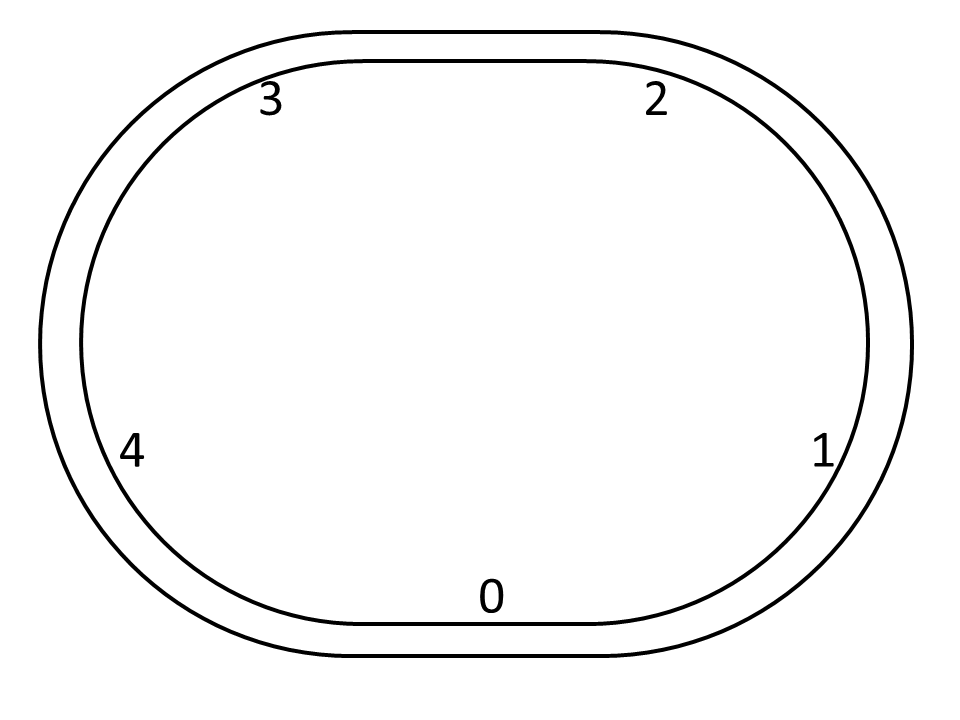
\includegraphics[width=2in]{images/racetrack.png}
\end{center}
\caption{5-mile racetrack}\label{fig:racetrack}
\end{figure}

Let's say the car starts at mile marker 0. The car may then travel forward (counterclockwise) or backwards (clockwise) any number of miles; we may define the car's  \emph{net displacement} as the the total number of forward miles traveled minus the the total number of backward miles. Net displacement is a very useful concept if you are a racecar driver. For example, the winner of the Indianapolis 500 is the the first driver to achieve a net displacement of 500 miles (in this case, only forward motion is allowed!)

We may characterize the displacement of the car using  
% \begin{center}
% ${\mathbb Z} = \{...,-3,-2,-1,0,1,2,3,...\}$. \\
% \end{center} 
a conventional number line, as shown in Figure~\ref{fig:displacement}. Moving forward around the racetrack corresponds to moving left (positive direction) on the number line; while moving backward around the racetrack corresponds to moving right (negative direction).
\begin{figure}[h]\label{fig:displacement}
\begin{center}
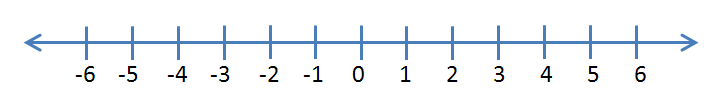
\includegraphics[width=4.5in]{images/integer_line.png}
\end{center}
\caption{Displacements on a 5-mile racetrack}
\end{figure}

\begin{exercise}{racetrack_displacements}
Compute the net displacement for the following multi-stage trips:
\begin{enumerate}[(a)]
\item
346 miles in the forward direction, then 432 miles in the backward direction, then 99 miles in the forward direction.
\item A forward displacements of 44 miles, followed by 13 additional forward displacements of 53 miles (one after the other).
\item Repeat the following sequence 25 times: a forward displacement  of 17 miles, followed by a backward displacement of 9 miles, followed by a forward displacement of 22 miles.
\end{enumerate}
\end{exercise}
From the preceding exercise, it appears that we may use ordinary addition, subtraction and/or multiplication to compute the car's net displacement after a trip involving several stages.

On the other hand, if we want to represent the \emph{position} of the car on the track as it relates to net displacement, we would have to relabel the number line as shown in  Figure~\ref{fig:positions}, using only the integers $0,1,2,3,4$.   
\begin{figure}[h]
\begin{center}
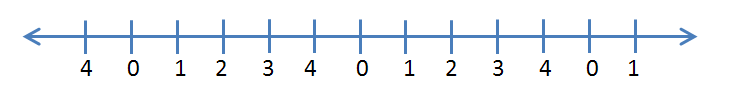
\includegraphics[width=4.5in]{images/integers_mod_5.png}
\end{center}
\caption{\label{fig:positions}Positions on the 5-mile racetrack}
\end{figure}

\begin{exercise}{racetrack_positions}
\begin{enumerate}[(a)]
\item
Compute the positions on the racetrack corresponding to each of the net displacements that you computed in Exercise~\ref{exercise:modular:racetrack_displacements}.
\item
How are your answers in (a) related to the corresponding answers in Exercise~\ref{exercise:modular:racetrack_displacements}?
\end{enumerate}
\end{exercise}

You may have noticed that different displacements correspond to the same position. For example, displacements of 8, 23, and -17 all correspond to the same position (namely 3). This prompts us to ask the question,  How can you tell when two displacements correspond to the same position?
One way to do this is make use of the answer to part (b) of Exercise~\ref{exercise:modular:racetrack_positions}. Most likely, you answered part (a) of Exercise~\ref{exercise:modular:racetrack_positions} by dividing the net displacements by 5 and taking the remainder. If two different net displacements correspond to the same position, then they have the same remainder when divided by 5.

We say that two displacements that correspond to the same position are \emph{equivalent}. For a 5-mile racetrack, for example, we have that 13 is equivalent to 18. We write this as: $13 \equiv 18 \pmod{5}$.

In general, if we're dealing with a situation that uses modulus $m$, then we define modular equivalence
as follows:

\begin{defn}\label{definition:modular:equivalence}
 Two integers $a$ and $b$ are \term{equivalent} mod $m$\index{Modular equivalence}  if both $a$ and $b$ have the same remainder when divided by $m$. To denote that $a$ and $b$ are \term{equivalent} mod $m$, we write: $a \equiv b \pmod{m}$.
 \end{defn}

\begin{rem}
This definition uses the notion of \emph{remainder},\index{Remainder} which we're assuming you're familiar with from  basic algebra. To be precise, the remainder of $a$ when divided by $m$ is a number $r$ between $0$ and $m-1$ such that  $a = q \cdot m + r$ for some integer $q$ ($q$ is called the ``quotient'').  In your basic algebra class you we always able to find a remainder for any division problem, and there was always just one right answer for the remainder. In other words, you found that the remainder always exists, and is unique. This ``basic" fact is actually not so easy to prove. It may be proved using the so-called \emph{division algorithm}.\index{Division algorithm}. You may find a proof in any book on number theory.
\end{rem}

\begin{rem}
Notice that Definition~\ref{definition:modular:equivalence} uses the 3-lined ``$\equiv$'' here instead of the usual $=$ sign. This notation is used  to emphasize the fact that modular equivalence resembles equality, but is not quite the same thing.  For example, we have already seen that 8 and 23 are equivalent mod 5, even though they are not equal.  In a later chapter we'll discuss equivalence relations, and we'll see that equivalence is in some sense a generalization of equality. For now,  be alerted to the fact that ``$\equiv$'' and ``$=$'' do not necessarily have the same properties. It's tempting for instance to make statements such as, ``$a \equiv b \pmod{m}$ implies $a-b \equiv 0 \pmod{m}$''. But just because this is true for $=$ doesn't mean it's also true for $\equiv$!  In this case the statement turns out to be true, but it requires proof -- and in this class you are not allowed to make assertions that have not been proven.\footnote{This may be one reason why not many mathematicians are politicians, and vice-versa.}  
\end{rem}

\begin{rem}
**(\emph{Important}) Many references use the expression ``$a \bmod m$'' to denote the remainder when $a$ is divided by $m$.  We prefer not to use this notation, since it can sometimes be confusing.  For example, according to this notation it is not true that $12 = 17 \bmod 5$, even though it is true that $12 \equiv 17 \pmod{5}$.   We will use instead the expression `` mod($a,m$)'' to indicate the remainder of $a$ when divided by $m$.  This is the notation used in most mathematical software (such as Excel and Matlab), and it reflects the fact that the remainder is a function of $a$ and $m$. 
\end{rem}

There is an alternative (and very useful) way to determine modular equivalence.
Suppose that $a \equiv b \pmod{m}$, so that $a$ and $b$ have the same remainder when divided by $m$. Let's call this remainder $r$. Then we can write  $a = p \cdot m + r$ and $b = q \cdot m + r$ for some integers $p,q$ It follows from basic algebra that $a - p \cdot m =b - q \cdot m$. We then proceed step-by-step using basic algebra as follows:
\begin{align*}
&a - p \cdot m = b - q \cdot m \\
\implies &\quad a - b = p \cdot m - q \cdot m \\
\implies &\quad a - b = (p - q) \cdot m. \\
\implies &\mbox{ $a - b$ is divisible by $m$}.
\end{align*}
In summary, we have shown that
\[\text{If } a \equiv b \pmod{m}  \text{ then } a - b \text{ is divisible by } m.\]
which we can also write as
\[a \equiv b \pmod{m} \implies \mbox{ $a - b$ is divisible by $m$.}\]
It turns out that the \emph{converse}\index{Converse} statement is also true.\footnote{In general, if you have a statement of the form ``If A then B'', then the converse  is ``If B then A''.  Similarly, the converse of ``A $\implies$ B'' is, ``B $\implies$ A''.}  The converse statement is: 
\[\mbox{ If  $a - b$ is divisible by $m$  then }a \equiv b \pmod{m}. \]
One way to prove this is to prove the \emph{contrapositive}, \index{Contrapositive} which is logically equivalent.\footnote{In general, the contrapositive of ``If A as true then B is also true'',  is ``If B is not true then A is not true''.  Alternatively: if you have a statement ``A $\implies$ B'', then the contrapositive is ``not B $\implies$ not A''. Unlike the converse, the contrapositive is \emph{always} true if the original statement is true} In this case, the contrapositive statement is, ``If $a \not\equiv b \pmod{m}$, then $a-b$ is not divisible by $m$'').

\begin{exercise}{equivdef}
Finish the proof of the contrapositive by filling in the blanks:

\noindent
Suppose $a \not\equiv b \pmod{m}$. Let $r$ be the remainder of $a$ when divided by \underline{~$<1>$~}, and let $s$ be  the remainder of \underline{~$<2>$~} when divided by \underline{~$<3>$~}. Since the remainders are unequal, it follows that one must be bigger than the other: let us choose $a$ to be the number with the larger remainder, so that $r > \underline{~<4>~}$. By the definition of remainder, we may write $a = p\cdot m + \underline{~<5>~}$, and we may also write $b = q\cdot \underline{~<6>~} + \underline{~<7>~}$. Then by basic algebra, $a - b = (p-q)\cdot \underline{~<8>~} + (r - \underline{~<9>~})$. 

We want to show that $r-s$ is the remainder of $a-b$ when divided by $m$. To do this, we need to show that $r-s$ is between 0 and $\underline{~<10>~}$. Since $r>s$ it follows that $r-s > \underline{~<11>~}$. Furthermore,
Since $r < m$ and $s \ge 0$, it follows that $r - s < \underline{~<12>~}$.  So we have shown that $r-s$ is between $\underline{~<13>~}$ and $\underline{~<14>~}$, so 
$r-s$ is the remainder of $a-b$ when divided by $m$. However, $r-s > 0$, which means that $a-b$ is not divisible by $\underline{~<15>~}$. This is exactly what we needed to prove, so the proof is complete. 
\end{exercise}

We summarize Exercise~\ref{exercise:modular:equivdef} and the preceding discussion together in the following proposition.

\begin{prop}{equivalence_alt}
Given any two integers $a$ and $b$, and a modulus $m$ ($m$ is a positive integer). Then 
\[
a \equiv b \pmod{m} \mathrm{~if~and~only~if~} a - b = k \cdot m,
\]
where $k$ is an integer.
\end{prop}
\noindent
We may rewrite Proposition~\ref{proposition:modular:equivalence_alt} more elegantly using mathematical shorthand as follows: Given $a,b,m \in {\mathbb Z}$, then 
\[
a \equiv b \pmod{m} \mathrm{~iff~} m | (a - b).
\]
Note the two shorthand expressions we have used here:  the symbol  `$\in$'  means `contained in' or `elements of', while the single vertical line `|' means ``divides'.


The following proposition establishes important facts about modular equivalence that we'll need later.\footnote{This proposition actually establishes that modular equivalence is  both \emph{transitive} and \emph{symmetric}. We'll talk more about transitive, symmetric relations in the Equivalence Relations chapter.}

\begin{prop}{equivalence_transitive}
Given any integers $a, b, c$ and a positive integer $n$ such that $a \equiv b \pmod{n}$ and $c \equiv b \pmod{n}$. Then it is also true that $a \equiv c, c \equiv a, b \equiv a,$ and $ b \equiv c$ (all these equivalences are $\pmod{n}$) .
\end{prop}
\begin{exercise}{eqproof}
Prove Proposition~\ref{proposition:modular:equivalence_transitive}. 
\hyperref[sec:modular_arithmetic:hints]{(*Hint*)}
\end{exercise}

\begin{exercise}{jan25}
Suppose January 25 is a Thursday. 
\begin{enumerate}[(a)]
\item
Use Definition~\ref{definition:modular:equivalence} to determine whether January 3 is a Thursday. Show your reasoning.
\item
Use Proposition~\ref{proposition:modular:equivalence_alt} to determine whether January 31 is a Thursday. Show your reasoning.
\item
Find the nearest Thursday to January 15. Show your reasoning.
\item
Find the nearest Thursday to April 18. Show your reasoning.  (Note: the year is not a leap year.)
\end{enumerate}
\end{exercise}

\begin{exercise}{22}
Determine whether or not the following equivalences are true. Explain your reasoning. If the equivalence is not true, change one of the numbers to make it true.
\begin{multicols}{2}
\begin{enumerate}[(a)]
 
\item
$71 \equiv 13 \pmod{4}$
 
 \item
 $-23 \equiv 13 \pmod{6}$

\item
$101 \equiv 29 \pmod{6}$

\item
$50 \equiv 13 \pmod{7}$

 \item
$654321 \equiv 123456  \pmod{5}$

 \item
$1476532 \equiv -71832778  \pmod{10}$
\end{enumerate}
\end{multicols}
\end{exercise}


Let us now return to the problem of finding the position corresponding to the net displacement following a multi-stage trip.
When you computed racetrack positions in Exercise~\ref{exercise:modular:racetrack_positions}, most 
likely you simply took the net displacements you computed in Exercise \ref{exercise:modular:racetrack_displacements}, divided by 5 and took remainder. 
However, our new concept of modular equivalence gives us another way of solving this problem -- one that can be much, much easier if we're dealing with large displacements.

\begin{example}{mod_add_new}
Suppose  Dusty drives around the 5-mile track 112 miles in a positive direction, then 49 miles in a negative direction, then 322 miles in a positive direction.  To find Dusty's net displacement we may take $112 - 49 + 322 = 385$ and then take the remainder mod $5$ (which turns out to be 0). But notice that:
\begin{align*}
112 &\equiv 2 \pmod{5},\\
-49 &\equiv 1 \pmod{5},\\
322 &\equiv 2 \pmod{5},\\
\end{align*}
and we compute
\[2 + 1 + 2 = 5 \equiv 0 \pmod{5}. \]
We have obtained the same answer with much less work. How did we do it? By \emph{replacing each number with its remainder}.
\end{example}

\noindent
Can we do the same thing with multiplication? 

\begin{example}{mod_mult_new}
Suppose I travel on my racetrack at a 113 miles per hour in the positive direction  for 17 hours. We may compute:
\begin{align}
&\text{Net displacement}: 113 \cdot 17 = 1921 \text{ miles} \notag\\
&\text{Final position}: 1921 = 384\cdot 5 + 1 \implies \text{final position} = 1. \notag
\end{align}
On the other hand, we may reach the same conclusion by a somewhat easier route:
\begin{align*}
113 &\equiv 3 \pmod{5},\\
17 &\equiv 2 \pmod{5},
\end{align*}
and we compute
\[3 \cdot 2 = 6 \equiv 1\pmod{5}. \]
Again, we have obtained the correct answer by \emph{replacing each number with its remainder}.
\end{example}

Does this work in general? In fact it does! However, this requires a mathematical proof.  We will discuss the proof in a later section -- but at least our discussion shows that \emph{arithmetic with remainders} is meaningful and useful.

If we're doing arithmetic $\pmod{n}$, then the remainders will necessarily be between $0$ and $n-1$ (inclusive). This set of  remainders has a special name, which later on we'll use extensively.

\begin{defn}\label{integers_mod_n}\index{Integers mod $n$}
The set $\{0,1,\ldots,n-1\}$ is called the \emph{integers mod $n$}, and is denoted by the symbol ${\mathbb Z}_n$.
\end{defn}

We will need the following proposition later:

\begin{prop}{equiv_mod_n}
Suppose $a,b \in  {\mathbb Z}_n$ and $a \equiv b \pmod{n}$. Then $a = b$.
\end{prop}

\begin{exercise}{27} 
Fill in the blanks in the following proof of Proposition~\ref{proposition:modular:equiv_mod_n}.

\noindent
We are given that $a,b \in  {\mathbb Z}_n$, which implies that $a \geq 0$ and $b \leq  \underline{~<1>~}$, so that $-b \geq  \underline{~<2>~}$.
It follows by adding these inequalities that $a - b \geq   \underline{~<3>~}$. 
Furthermore, since $a,b \in  {\mathbb Z}_n$, we have $a \leq \underline{~<4>~}$ and $b \geq  \underline{~<5>~}$, so that $-b \leq  \underline{~<6>~}$.
It follows by adding these two results that $a - b \leq  \underline{~<7>~}$. In other words,  $a - b$ is between $\underline{~<8>~}$ and $\underline{~<9>~}$. 

Furthermore, we were given that $a \equiv b \pmod{n}$. It follows from Proposition~\ref{proposition:modular:equivalence_alt} that $\underline{~<10>~}$ is  a multiple of $\underline{~<11>~}$. 
The only multiple of $\underline{~<12>~}$ between $\underline{~<13>~}$ and $\underline{~<14>~}$ is $\underline{~<15>~}$, so that $a - b = \underline{~<16>~}$. It follows by algebra that $a = \underline{~<17>~}$, and the proof is complete.
\end{exercise}


\begin{exercise}{28}
Now you're ready! Give answers for the seven examples at the beginning of this chapter.
\end{exercise}

\section{Modular equations}\label{section:modular:ModularEquations}

\subsection{More uses of modular arithmetic  }
 
Supermarkets and retail stores have a dirty little secret. Every time you scan your purchases, they're using modular arithmetic on you! In fact, modular arithmetic is the basis for UPC and ISBN bar codes. We will use these practical examples to introduce \emph{modular equations}\index{Modular equations}. 

\begin{figure}
\begin{center}
\centerline {
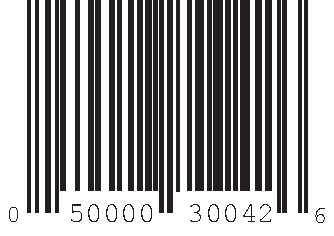
\includegraphics[width=2in]{images/UPCcode.pdf}
}
\end{center}
\caption{A UPC code}
\label{groups_figure_3}
\end{figure}


\begin{exercise}{UPCSymbols} \emph{Universal Product Code}
\index{Code!UPC} (UPC) symbols are now found on most \index{UPC code}
products in grocery and retail stores. The UPC symbol (see Figure~\ref{groups_figure_3}) is a 12-digit
code which identifies the manufacturer of a product and the product itself. The first 11 digits contain the information, while the twelfth digit is used to check for errors that may occur while scanning. If $d_1 d_2
\cdots d_{12}$ is a valid UPC code, then  
\[
3 \cdot d_1 + 1 \cdot d_2 + 3 \cdot d_3 + \cdots + 3 \cdot
d_{11} + 1 \cdot d_{12} \equiv 0 \pmod{10}.
\]
So the scanning device that cashiers use reads the code and adds up the numbers mod 10. If they don't add to zero, then the device knows it hasn't scanned properly. 
(Smart little bugger, that scanner is!)

\begin{enumerate}[(a)]
\item
Show that the UPC number  0-50000-30042-6, which appears in
Figure~\ref{groups_figure_3}, is a valid UPC number. 
 
\item
Show that the number 0-50000-30043-6 is not a valid UPC number.
 
\item (\emph{for geeks}) Write a program or Excel spreadsheet that will determine whether or not a UPC number is valid. 

\item
One common scanning error occurs when two consecutive digits are accidentally interchanged. This is called a \term{transposition error}.\index{Transposition!error} 
The  UPC error detection scheme can catch most transposition errors.  Using the UPC in (a) as the correct UPC, show that the transposition error 0-50003-00042-6 is detected.  Find a transposition error that is not detected. 

\item
 Using the UPC in (a) as the correct UPC, show that the single-digit error 0-50003-30042-6 is detected.  
\item
**Prove that the UPC error detection scheme detects all single digit errors. 
\hyperref[sec:modular_arithmetic:hints]{(*Hint*)}   
\end{enumerate}
\end{exercise} 
 

It is often useful to use an \term{inner product} notation\index{Inner product!notation} for these types of error detection schemes.\footnote{You may have seen inner products (a.k.a. ``dot products'') in one of your math classes talking about vectors.} In the following text, the notation
\[
(d_1, d_2, \ldots, d_k ) \cdot (w_1, w_2, \ldots, w_k ) \equiv 0 \pmod{ n }
\]
will be used to mean
\[
d_1 w_1 +  d_2 w_2 + \cdots +  d_k w_k  \equiv 0  \pmod{ n}.
\]

\begin{exercise}{ISBNCodes}
Every book has an \emph{International Standard Book Number}\index{Code!ISBN} (ISBN-10) code\index{Error detection codes!ISBN}.  This is a 10-digit code indicating the book's language, publisher and title. The first digit indicates the language of the book; the next three identify the publisher; the next five denote the title; and the tenth digit is a check digit satisfying 
\[
(d_1, d_2, \ldots, d_{10} ) \cdot (1, 2, \ldots, 10 )  \equiv 0 \pmod{11}.
\]
ISBN-10 codes are nice in that all single-digit errors and most transposition errors can be detected.  One complication  is that $d_{10}$ might have to be a 10 to make the inner product zero; in this case, the character `X' is used in the last place to represent 10.

\begin{enumerate}[(a)]
 
\item
Show that 3-540-96035-X is a valid ISBN-10 code. 

\item
Is  0-534-91500-0 a valid ISBN-10 code?  What about 0-534-91700-0 and 0-534-19500-0? 
 
 \item
How many different possible valid ISBN-10 codes are there?

\item
Write a formula of the form $d_{10} \equiv \ldots \pmod{\ldots}$  to calculate the check digit in an ISBN-10 code. 
\hyperref[sec:modular_arithmetic:hints]{(*Hint*)}

\item
*Prove that any valid ISBN-10 code also satisfies:
\[
(d_1, d_2, \ldots, d_{10} ) \cdot (10, 9, \ldots, 1 )  \equiv 0 \pmod{11}.
\]

\item
* Prove that if  $(d_1, d_2, \ldots,d_9,  d_{10} )$ is a valid ISBN-10 code, then $(d_{10}, d_9, \ldots, d_2, d_1 )$  is also a valid ISBN-10 code (as long as $d_{10}$ is not equal to X).
  
 \item
(\emph{for geeks}) Write a computer program or Excel spreadsheet that calculates the check digit for the first nine digits of an ISBN code. 
 
 \item
A publisher has houses in Germany and the United States.  Its German prefix is 3-540.  Its United States prefix will be 0-{\it abc}.  Find four possibilities for {\it abc} such that the rest of the ISBN code will be the same for a book printed in Germany and in the United States.  

\item
**Prove that the ISBN-10 code detects all single digit errors.
\hyperref[sec:modular_arithmetic:hints]{(*Hint*)}

\item
**Prove that the ISBN-10 code detects all transposition errors. 
\hyperref[sec:modular_arithmetic:hints]{(*Hint*)}

\end{enumerate}
\end{exercise}



%We've already seen, or needed the use of, a couple modular equations.  For instance in the last subsection, we developed and/or used modular equations for 1c, 1d, 2d, 2e, and 2f.  Looking at the term modular equation, what would you guess it means? An equation using modular arithmetic?  Perfect.  The following are good examples of modular equations:
%\[
%(3 \cdot d_1) + (1 \cdot d_2) + (3 \cdot d_3) + \cdots + (3 \cdot
%d_{11}) + (1 \cdot d_{12}) \equiv 0 \pmod{10}.
%\]
%\[
%(d_1, d_2, \ldots, d_{10} ) \cdot (10, 9, \ldots, 1 )  \equiv 0 \pmod{11}.
%\]

%These were the error detection schemes for UPC's and ISBN codes in Exercises \ref{exercise:modular:UPC_Symbols} and \ref{exercise:modular:ISBN_Codes} respectively.  Notice that there are variables, unknowns to solve for or fill in for these equations.  We know from algebra that an equation doesn't have to involve unknowns; it simply has to state an equality between two mathematical expressions.  But equations are no fun unless you have to solve for something.  So when we speak of modular equations, we're referring to ones in which there is an unknown to solve for.  And notice the use of the $ \equiv $ sign in the equations.  Equivalence is a generalized form of equality, therefore when we speak of modular equations, we're speaking of ones that use an $ \equiv $ sign.


\subsection{Solving modular equations}

In Exercise ~\ref{exercise:modular:ISBNCodes} part (h) you solved a modular equation with three variables by trial and error: you couldn't solve for one variable at a time, so you had to test out sets of values for $a$, $b$, $c$ together and see if the the ISBN equation held.  The UPC and ISBN error detection schemes themselves, given again below,  are examples of modular equations with 12 and 10 variables, respectively: 

\[
(3 \cdot d_1) + (1 \cdot d_2) + (3 \cdot d_3) + \cdots + (3 \cdot
d_{11}) + (1 \cdot d_{12}) \equiv 0 \pmod{10}.
\]
\[
(d_1, d_2, \ldots, d_{10} ) \cdot (10, 9, \ldots, 1 )  \equiv 0 \pmod{11}.
\] 

Can the above equations be solved?  You may remember from college algebra that you can't uniquely solve a single equation for 10 or 12 variables.\footnote{Actually, there are many possible combinations of 10 or 12 variables which make the equations work.}  But if we supply additional information so that only variable is left to solve for, then we can use the resulting equation to find the value of the variable.  Let's try.  

\begin{exercise}{check_digit}
Suppose you're given the following UPC:  1-54637-28190-?.  Write a modular equation to solve for the missing check digit, then solve it.
\end{exercise}{}

In the preceding exercise you should have come up with an equation that looks like:
\[
(3 \cdot 1) +  \ldots + (3 \cdot 0) + (1 \cdot x) \equiv 0 \pmod{10}.
\]

How did you solve this?  One possible method is to add up all the terms the left side of the equation short of the variable, and then figure out how much you need to add to that sum to get a number divisible by $10$. Keep this method and your own method (if different) in mind, as they are good intuition on how to solve these problems in general.

Is there a \emph{unique} answer for $x$?  Practically, for a UPC code $x$ must be between $0$ and $9$ (that is, $x \in {\mathbb Z}_{10}$: with this restriction, there is indeed only one solution.  But if we remove that restriction, then there are many solutions.  For instance $x=12$ and $x =22$ both work (check this for yourself).  Can you think of any other integers that work? 

%But notice that the equation involves an equivalence sign rather than an equals sign.  if we removed that restriction, are there other solutions to the equation?  If the equation involved an ''$=$" sign, $x = 2$ would be the only solution.   Now if we remove the restriction that $x \in {\mathbb Z}_n$, then $x=2$ is not the only solution for the problem.  In other words, if if we don't restrict the $x$ in the equation to being a number $0-9$, Since we're dealing in mod 10, $x=12$ would also work (check this to convince yourself).  Can you think of any other integers that work? 

In fact any integer equivalent to $2 \pmod{10}$ also works.  But from our intuitive methods, would we have come up with these other possible solutions?  In most cases not.  Therefore we need to come up with a general method that will give us all possible integer solutions of a modular equation.  Just as in basic algebra, we'll start with simpler equations and move to more complicated ones. 

\begin{example}{mod_eq_add}
%%% CPT I'm not sure we want to separate out addition equations.
Let's start with a basic modular equation involving addition: \index{Modular equations!addition}
\[
8 + x \equiv 6 \pmod{11}
\]

From algebra we understand how to solve an equation with an $=$ sign, but what do we do with this $ \equiv $ sign?  In fact, we can turn it in to an $=$ sign by using Proposition~\ref{proposition:modular:equivalence_alt}, which says that $8 + x \equiv 6 \pmod{11}$ means the same as:
\[
8 + x = k \cdot 11 + 6
\]
And then we can solve for $x$ like any other equation.  The result is
\[
x = k \cdot 11 - 2
\]
So we solved for $x$, but  what numbers does $x$ actually equal?  What does $k \cdot 11 - 2$ mean?  $k$ is an integer, therefore $x$ can equal -2 (if $k = 0$), or -13 (if $k = -1$), or 9 (if $k = 1$), and so on.  In other words $x$ equals $-2$ plus any integer multiple of $11$, which, by the definition of modular equivalence, means
\[
x \equiv -2 \pmod{11}
\]
This is a correct solution: but it's not the only way to write it. It would be just as valid to write
\begin{itemize}
\item
$x \equiv -13 \pmod{11}$
\item
$x \equiv  20 \pmod{11}$
\item
$x \equiv  130 \pmod{11}$
\item
$\ldots$
\end{itemize}
Notice however that there is only one way to write the solution in terms of a number in ${\mathbb Z}_{11}$, namely:
\[
x \equiv 9 \pmod{11}
\]
In order to avoid ambiguity, mathematicians and textbooks always write solutions mod $n$ in terms of numbers in ${\mathbb Z}_n$. 
In our current example, it's easy enough to obtain the standard solution ($x \equiv 9 \pmod{11}$)  directly from the equation $x = k \cdot 11 - 2$? by taking
one of the $11$'s and adding it to the $-2$ to get
\[
x = (k-1) \cdot 11 + 11 - 2 = (k-1) + 9,
\]
giving  $x \equiv 9 \pmod{11}$.

\end{example}

\medskip

\noindent
To summarize our general method for solving modular equations so far:

\begin{enumerate}
\item
Turn the $ \equiv $ sign into an $=$ sign using the definition of modular equivalence. This introduces an additional variable $k$.
\item
Find (by trial and error if necessary) the value of $k$ that puts $x$ in the appropriate range.
\item
Change the equation back into an equivalence.
\end{enumerate}


\begin{exercise}{mod_eq_1}
Find all $x \in {\mathbb Z}$ satisfying each of the following equations.

\begin{enumerate}[(a)]
\item
$5 + x \equiv 1 \pmod{ 3}$
\item
$25 + x \equiv 6 \pmod{ 12}$
\end{enumerate}
\end{exercise}

Now let's spice things up with some multiplication:

\begin{example}{mod_eq_mult1} Given the equation
\[
5x + 3 \equiv 9 \pmod{11}.
\]

\noindent
Using the definition of modular equivalence, this becomes
\[
5x + 3 = 11k + 9.
\]

\noindent
Solving this equality using basic algebra gives us 
\[
x = \frac{11k + 6}{5}. 
\]

Now remember that $x$ must be an \emph{integer}.  In order for the right side to be an integer, we need to find a $k$ that makes $\frac{11k+6}{5}$ an integer. At this point we may use trial and error to find a $k$ in ${\mathbb Z}_5$ such that $11 \cdot k + 6$ is a multiple of $5$. We get $k=4$; and in fact adding $5\cdot n$ to 4 also works for any $n \in {\mathbb Z}$, since $5n$ is always divisible by $5$.  Now we can solve for $x$ by substituting $k=4+5n$ back in to the previous equation:

\begin{align*}
x =& \dfrac{11(4 + 5\cdot n) + 6}{5} \\
&=\dfrac{11\cdot 4 + 6}{5} + \dfrac{11 \cdot (5 n)}{5} \\
& = 10 + 11 n 
\end{align*}
Therefore $x \equiv 10 \pmod{11}$ is the general solution.  You may check (which is always a good idea!) by plugging $10 + 11n$ for a couple values of $n$ back into the original equation, and you'll see these numbers work.
\end{example}


%\]
%which is an integer for any $n \in {\mathbb Z}$ .  Therefore $k$ can be $1$ plus  any integer multiple of $5$, that is $k = 1 + 5n$: and the corresponding solution for $x$ is
%\[
%x = 4 + 11n.
%\]


Just to make sure you've mastered the process, we'll give another example:

\begin{example}{mod_eq_mult2}
To solve the equation $4x + 5 \equiv 7 \pmod{11}$ we proceed step by step (note that the symbol $\implies$ is mathematicians' shorthand for ``implies''):
\begin{align*}
&4x + 5 \equiv 7 \pmod{11} \\
 \implies &4x + 5 = 11k + 7&\text{(by modular equivalence)}\\ 
\implies &x = \dfrac{11k + 2}{4}&\text{(basic algebra)}
\end{align*}
Now, $11k + 2$ is a multiple of $4$ when $k = 2$, as well as when $k$ equals $2$ plus any multiple of $4$. 
Therefore $k = 2 + 4n$, hence we may continue from the previous equation:

\begin{align*}
&x = \dfrac{2 + 11k }{4}\\
\implies &x = \dfrac{ 2 + 11 \cdot (2 + 4n)}{4} &\text{(substitution)} \\
\implies &x = 6 + 11n. &\text{(simplification)}
\end{align*}
\end{example}

\begin{rem}
Example~\ref{example:modular:mod_eq_mult2} demonstrates some good practices that you can make use of when you write up your own proofs:
\begin{itemize}
\item
Instead of using a sentence to explain your reasoning for each step, place the reason to the right (like I did).  This shrinks down the size of the proof.
\item  
Another way to shrink the proof is to use mathematical equations, expressions, and symbols (such as $\implies, \forall$) whenever you can to accurately communicate your steps in the proof.  
\end{itemize}
\end{rem}



In summary, a general method for solving modular equations is:

\begin{enumerate}[1.]
\item
Turn the $ \equiv $ sign into an $=$ sign using the definition of modular equivalence (just as with modular addition). This introduces another constant $k$.
\item
Solve the resulting equation for your variable $x$. If the expression is a fraction, then
 go to step $5$.
Otherwise, go to step $3$.
\item
By trial and error, find a value $k_0$ for $k$ which makes the fraction into an integer.
\item
Substitute  $k_0$ + $n \cdot$(denominator) in for $k$, and simplify.
\item
Change the equation back into an equivalence.
\end{enumerate}

\begin{exercise}{mod_eq_2}
Find all $x \in {\mathbb Z}$ satisfying each of the following equations. (If there's no solution, then you can say ``no solution''-- but show why!)

\begin{multicols}{2}
\begin{enumerate}[(a)]
\item
$9x \equiv 3 \pmod{ 5}$
\item
$5x \equiv 1 \pmod{ 6}$
\item
$7x \equiv 9 \pmod{ 13}$
\item
$8x \equiv 4 \pmod{ 12}$
\item
$11x \equiv 2 \pmod{ 6}$
\item
$27x \equiv 2 \pmod{ 9}$
\item
$3 + x \equiv 2 \pmod{ 7}$
\item
$5x + 1 \equiv 13 \pmod{ 23}$
\item
$5x + 1 \equiv 13 \pmod{ 26}$
\item
$3x + 2 \equiv 1 \pmod{ 6}$  
\end{enumerate}
\end{multicols}
\end{exercise}


One major disadvantage of our solution method is the use of trial and error in step $3$. If large numbers are involved, then this step can take a long time. However, there are techniques to speed things up:

\begin{example}{speed_up1}
Consider the equation $79x \equiv 9 \pmod{15}$. In Section~\ref{sec:ModEquiv} we mentioned that when we're doing arithmetic mod $n$, we can replace any number with its remainder mod $n$ without changing the answer. In this example then, we can replace the 79 with its remainder mod 15, which is 4. Thus we have
\[ 4x \equiv 9 \pmod{15}, \]
which leads to 
\[ x = \dfrac{15k +9}{4}. \]
By rewriting the numerator, we can simplify the right-hand side:
\[ x = \dfrac{(12k + 3k) + (8 + 1)}{4} = 3k + 2 + \dfrac{3k + 1}{4}. \]
and we readily discover that $k=1 + 4n$ makes the right-hand side an integer, so that 

\begin{center}
$x = \dfrac{15\cdot(1+4n) +9}{4} = 6$, or $x \equiv 6 \pmod{15}$.
\end{center}

% By following our procedure, we first convert this to $78x = 15k + 9$. If we solve this for $x$ as before, we get
% \[
% x = \dfrac{15k +9}{4},
% \]
% and finding a $k$ which yields an integer might take some time!  However, note that $78 = 5\cdot 15 + 4$, so we may rewrite $78x = 15k + 9$ as 
% $15\cdot 5x + 4x = 15k + 9$. We may rearrange to obtain  $4x = 15(k-5x) + 9$, or
% \begin{align}
% x &= \dfrac{15(k-5x)}{4} + \frac{9}{4} = \left( 3(k-5x) + \dfrac{3(k-5x)}{4} \right) + \left( 2 + \frac{1}{4} \right) \\
% &=  3(k-5x) + 2 +  \dfrac{3(k-5x)+1}{4}.
% \end{align}
% At this point, to get a solution for $x$ we must choose $k-5x$ so that $3(k-5x)+1$ is divisible by $4$. This requires that $(k-5x) = 1 + 4n$, which gives the following expression for $x$:
% \begin{equation*}
% x = 3(1+4n) + 2 +  \dfrac{3(1+4n)+1}{4} = 5 + 12n + 1 + 3n = 6 + 15n,
% \end{equation*}
% which implies $x \equiv 6 \text{ (mod 15)}$ is the solution.
\end{example}

Just one more similar example:

\begin{example}{speed_up2}
To solve the equation $447x + 53 \equiv 712 \pmod{111}$ we proceed as follows:
\begin{align*}
447x + 53 \equiv& 712 \pmod{111} \\
\implies 3x + 53 \equiv& 46 \pmod{111} &\text{(modular equivalence)} \\
 \implies 3x + 53 =& 46 + 111k &\text{(modular equivalence)}\\ 
 \implies 3x  =& -7 + 111k &\text{(basic algebra)}\\ 
 \implies x =& \frac{-7 +111k}{3} &\text{(basic algebra)}\\
 \implies x =& \frac{-7}{3} + 37k &\text{(basic algebra)}
 \end{align*}
It should be clear that no value of $k$  makes the right side an integer.  Hence $x$ has no solution. You may have run into a similar situation in a previous exercise.
\end{example}

\begin{exercise}{modeq3}
Find all $x \in {\mathbb Z}$ satisfying each of the following equations.
\begin{multicols}{2}
\begin{enumerate}[(a)]
\item
$112x \equiv 2 \pmod{ 6}$
\item
$74x \equiv 9 \pmod{ 13}$
\item
$856x \equiv 4 \pmod{ 123}$ 
\hyperref[sec:modular_arithmetic:hints]{(*Hint*)}
\item
$272x \equiv 24 \pmod{ 9}$
\item
$242x + 39 \equiv 489 \pmod{236}$
\item
$469x + 122 \equiv 1321 \pmod{ 231}$
\item
$246x + 200 \equiv 401 \pmod{ 81}$
\item
$339 + 411x \equiv 2 \pmod{ 297}$
\item
$530x - 183 \equiv 215 \pmod{ 128}$ 
\end{enumerate}
\end{multicols}
\end{exercise}

From parts (h) and (i) of Exercise \ref{exercise:modular:modeq3} we see that even our trick with modular equivalences doesn't make all modular equations easy to solve.  When the coefficient of $x$ and the modulus are both large, you may end up needing \emph{lots} of trial and error.  And mathematicians are a bit snobby: we prefer solution methods that don't require \emph{any} trial and error.  There is actually a method that both eliminates trial and error and solves \emph{any} modular equation: this is the Euclidean algorithm, which we'll discuss later.

% \begin{exercise}{}
% Find all $x \in {\mathbb Z}$ satisfying each of the following equations.

% \begin{multicols}{2}
% \begin{enumerate}[(a)]
% \item
% $339 + 411x \equiv 2 \pmod{ 297}$
% \item
% $469x + 122 \equiv 1321 \pmod{ 231}$
% \item
% $530x - 183 \equiv 215 \pmod{ 128}$
% \item
% $246x + 200 \equiv 401 \pmod{ 81}$
% \end{enumerate}
% \end{multicols}
% \end{exercise}


%Credit card companies, banks, book publishers, and supermarkets all
%take advantage of the properties of integer arithmetic modulo $n$ and
%group theory to obtain error detection schemes for the identification
%codes that they use. The following two exercises present two familiar identification codes.

%The integers mod $n$ have become indispensable in the theory and applications of algebra.  Practical uses include cryptography, coding theory, and in identification codes.  In this section we'll focus on the use of integers mod $n$ in identification codes.

%this discussion should be expanded. We should make them give the proof. 

%%% Following is original discussion, which is replaced
% Suppose that on your way to work, an alarm on your phone goes off letting you know that 12 hours from now the turkey must be taken out of the oven.  It is currently 7 o� clock in the morning.  At what time will you take the turkey out of the oven?  Seven in the evening; right.  Why not 19 o' clock?  How do we take 7, add 12, and get 7?  

% What we in fact do is recognize that our system of telling time relies on two \textbf{\emph{cycles}} of 12 hours in a day; every 12 hours, the number, or name, of the hour is the same.  10 A.M. is 12 hours after 10 P.M., but the numerical label, 10, is the same.  

% And if you take a second to think about it, mathematically, what we're doing is we add 7 and 12 to get 19, and \emph{then} divide 19 by 12; our remainder, 7, is the hour we take the turkey out.  So we're not using simple addition; we�re using a modified addition, where we divide the result of the addition by a certain number (the size of our �cycle�), and the result we're looking for is the remainder of that division.

% \begin{example}{1}
% For instance, lets say you get up at 5 in the morning to prep the turkey, and you get it in the oven at 6.  You are cooking it low and slow to keep it juicy, so you decide to cook it for 14 hours.  At what time will you take it out of the oven?   

% As mentioned above, there are two slightly different but equivalent ways to think through this problem: 

% \begin{itemize}
% \item
% \underline{Method 1}: First, we rewrite 14 as:
% \[
% 14 = 12 + 2 = [\text{1 cycle}] + 2;
% \]
% Then we add: 
% \[
 % 6 + 14 = 6 + ([\text{1 cycle}] + 2) = [\text{1 cycle}] + 6 + 2 = [\text{1 cycle}] + 8
% \]
% Since [1 cycle] doesn't change the time on the clock, we have our answer:  \textbf{8 o'clock}.

% \item
% \underline{Method 2}: First, we add:
% \[
% 6 + 14 = 20;
% \]
% Then we use division with remainder:
% \[
 % 20|12 = 112 + 8. 
% \]
% Once again, the time on the clock is \textbf{8 o'clock}.
% \end{itemize}
% \end{example}

% \begin{example}{2} {\it (Continued from previous example)} 
% Now on second  thought, you realize as you put the turkey in that the family is coming in for an early supper.  So you decide to cook it at 50 degrees higher for 8 hours, instead of 14 hours.  At what time will you take the turkey out of the oven?  

% Again, there are (at least) a couple of ways to think through this:

% \begin{itemize}
% %\newline
% \item
% \underline{Method 1}: We're starting at 6 o'clock, so we have 6 hours left until noon. We're going to be cooking 8 hours, so we rewrite 8 as:
% \[
% 8 = 6 +2; 
% \]
% Therefore, 
% \[
% 6 + 8 = 6 + (6 +2) = 12 + 2 = [\text{1 cycle}] + 2
% \]
% Since [1 cycle] doesn't change the time on the clock, we have our answer:  \textbf{2 o'clock}.

% \item
% \underline{Method 2}: First, we add:
% \[
% 6 + 8 = 14; 
% \]
% Then we use division with remainder:
% \[
% 14|12 = 1\cdot 12 +2
% \]
% Once again, the clock time is \textbf{2 o'clock}.
% \end{itemize}
% \end{example}

 % If you take a second to look at these two examples, you will realize that Method 2 is an example of a general rule: 
% \begin{itemize}
% \item
% add the current hour to the number of hours in the oven, 
% \item
% divide by 12, and the remainder after division is your answer.  
% \end{itemize}

% We'll call this procedure "modified" addition. So no matter whether you're dealing with adding less than or more than 12 hours, this ''modified'' addition is a nice, tidy mathematical way to solve the problem that works every time. 

% To summarize in general: if $a$ represents the current hour, $b$ represents the number of hours added,  and $m$ represents the number of hours in the cycle (12), then the ``modified`` sum $a +_m b$ is equal to the remainder of $a+b$ when it's divided by $m$.  In other words:

% \[
% a +_m  b = r \mathrm{~iff~} a + b = k \cdot m + r
% \]
% where $k$ is an integer, and  $r$ is a nonnegative integer less than $m$ (Recall that ``iff'' is mathematicians' shorthand for ``if and only if'').

% You will see in the following exercises that this "modified" addition is actually quite practical in a number of different situations.

% \begin{exercise}{modex1}
% If today is Wednesday, what day of the week will it be 23 days from now?
% \end{exercise}
% \begin{exercise}{modex2}
% If today is the 2nd of October, what day of the month will it be 55 days from now?
% \end{exercise}
% \begin{exercise}{modex3}
% A lunar year is 354 days. If Chinese New Year is determined according to the lunar year, and Chinese New Year is February 14 in 2010, then when is Chinese New Year in 2011? When is Chinese New Year in 2012? 
% \footnote{Note that the Chinese calendar actually adds extra months in some years, so not every Chinese year is 354 days.}
% \end{exercise}
% \begin{exercise}{modex4}
% A car is at the 155 mile mark of a 250-mile circuit.  It drives another 425 miles.  What mile mark is it at now?
% \end{exercise}
% \begin{exercise}{modex5}
% A  car has had three owners. The first owner drove the car 89,000 miles. The second owner drove 57,000 miles. The third owner drove 92,000 miles. The third owner now tries to sell it to you. What is the mileage showing on the odometer (the odometer only goes up to 99,999).
% \end{exercise}
% \begin{exercise}{modex_last}
% $m\angle A = 54^o$. If $\angle A$ is increased by $900^o$, then what $m\angle A$?
% \end{exercise}

% \subsection{Modular addition}

% This ''modified'' addition we've been speaking of is actually called \term{modular addition}\index{Modular addition}.  The size of one cycle (which we've denoted as $m$) is called the \term{modulus}\index{Modulus!in modular addition}.  So modular addition refers to  addition done according to a modulus: that is, addition in which the numbers reset (or cycle around) every time you reach the modulus.

% \begin{exercise}{}
% Give the modulus used in  Exercises~\ref{exercise:modular:modex1} through~\ref{exercise:modular:modex_last}.
% \end{exercise}

% Previously we used $a+_m b = r$ to denote an equation in our "modified" addition. In conventional math books though, modular addition \index{Modular addition!definition} equations are usually written as:

% \begin{center}
% $a + b = r \pmod{m}$
% \end{center}
% In math books, you may see questions like:

% \begin{center}
% What is 7 + 88 (mod 12)? \\
% \end{center}
% \medskip{}

% \noindent
% What they're asking for is the solution to:

% \begin{center}
% 7 + 88 = $x$ (mod 12), \\
% \end{center}
% which is $x = 11$, since $7+88 = 4 \cdot 12 + 11$.

% \begin{exercise}{}
% Write the mathematical equations  corresponding to Exercises~\ref{exercise:modular:modex1} through~\ref{exercise:modular:modex_last}.
% \end{exercise}
% \begin{exercise}{}
% \begin{enumerate}[(a)]
% \item
 % Does 22+13 = 9 (mod 16)?  Why or why not?  Change the problem if necessary so that it is correct.
% \item
% Does 45+125 = 25 (mod 30)?  Why or why not?  Change the problem if necessary so that it is correct.
% \end{enumerate}
% \end{exercise}
% \begin{exercise}{ex1}
% \begin{multicols}{2}
% \begin{enumerate}[(a)]
% \item
% What is 12+13 (mod 17)? 
% \item
% What is 12+13 (mod 8)? 
% \item
% What is 1200+1300 (mod 800)?
% \end{enumerate}
% \end{multicols}
% \end{exercise}
% So far we've been looking at expressions of the form $a + b \pmod{c}$, but there's no reason we can't generalize. For instance,  Exercise~\ref{exercise:modular:ex1}(b) could have been phrased, "What is 25 (mod 8)?"  The answer is the same.

% \begin{exercise}{}
% \begin{multicols}{2}
% \begin{enumerate}[(a)]
% \item
% What is 261 (mod 16)? 
% \item
% What is -400 (mod 21)? 
% \item
% What is $2^{1024} \pmod{32}$?
% \end{enumerate}
% \end{multicols}
% \end{exercise}


% \subsection{Modular equivalence}

% Suppose a  car is driving around a 5-mile track, and you're there to take pictures of it.  The car leaves the starting line at the wave of the checkered flag, and the first snapshot you take of the car occurs after it has traveled three miles.  The second snapshot is taken after it has traveled 8 miles.  When you develop and look at these two pictures, will you be able to tell them apart?  

% In fact, they will look exactly the same. At 8 miles the car is in the same position as it was at 3 miles, precisely because the car is driving around a 5-mile track.  For that matter, the car will be in the same position on the track after 13 miles, 18 miles, 23 miles, etc.  Of course you can tell which one is which by their order on the film (or in your digital camera).  But if I handed you the pictures out of order and with no labels, you couldn't tell which is which.  So what we could say is that these pictures, or miles, are essentially the same. How can you explain this situation in terms of the modular terminology we've been developing?

% \begin{exercise}{}
% Fill in the blanks in the following explanation:  ``On a 5-mile track, the car looks the same after $3,8,13,18\ldots$ because: 
% \begin{eqnarray*}
% 8 \pmod{\_\_\_\_} &= 3, \\
 % 13 \pmod{\_\_\_\_} &= \_\_\_\_,\\
% \text{and~} \_\_\_\_ \pmod{\_\_\_\_} &= \_\_\_\_.
% \end{eqnarray*}
% \end{exercise}

% \begin{exercise}{}
% \begin{enumerate}[(a)]
% \item
% Give ten numbers that are equal to $3 \pmod{5}$
% \item
% Give ten numbers that are equal to $7 \pmod{13}$
% \end{enumerate}
% \end{exercise}

% Continuing with our racetrack example, we can say that $3,8,13,\ldots$ are all \emph{equivalent} mod 5; they're all the same, as judged by a modulus of 5.  This leads to our first definition of \term{modular equivalence} \index{Equivalence!modular!first definition}\index{Modular equivalence}.

% \begin{defn}\label{mod_equiv_def_1} \emph{(modular equivalence, first definition)}
% $a \equiv b \pmod{m}$ iff $a \pmod{m} = b \pmod{m}$
% \end{defn}

% \begin{exercise}{}
% \begin{multicols}{2}
% \begin{enumerate}[(a)]
% \item
% Is $-22 \equiv 3 \pmod{5}$?
% \item
% Is $46 \equiv 4 \pmod{6}$?
% \item
% Is $380 \equiv 136 \pmod{6}$?
% \end{enumerate}
% \end{multicols}
% \end{exercise}

% We can write Definition~\ref{mod_equiv_def_1} another way using division with remainder.  Recall that $a \pmod{m} = r$ means that
% \[a = p \cdot m + r \]
% for some integer $p$, which is the same as saying that
% \[a - p \cdot m = r. \]
% Similarly, $b \pmod{m} = r$ means that
% \[b - q \cdot m = r \]
% for some integer $q$. Since the two right hand sides are equal, we can set the left hand sides equal:
% \[a - p \cdot m = b - q \cdot m  \]
% Rearranging gives:
% \[a - b = (p - q) \cdot m  \]
% To summarize: we have shown that $a \equiv b \pmod{m}$ implies that $a-b$ is divisible by $m$. It turns out that the reverse is true as well:
% if $a-b$ is divisible by $m$, then $a \equiv b \pmod{m}$:

% \begin{exercise}{equivdef}
% Show that if $a-b$ is divisible by $m$, then $a \equiv b \pmod{m}$.
% \end{exercise}

% The above results enable us to give a second definition of modular equivalence \index{Equivalence!modular!second definition} which is very useful:


% \begin{defn}\label{mod_equiv_def_2} \emph{modular equivalence, second definition)}
% \[
% a \equiv b \pmod{m} \mathrm{~iff~} a - b = k \cdot m,
% \]
% where $k$ is an integer (that is, $k \in  {\mathbb Z}$). Alternatively, 
% \[
% a \equiv b \pmod{m} \mathrm{~iff~} a  = b + k \cdot m.
% \]
% \end{defn}
% We now have two ways to decide whether or not two numbers are equivalent mod $m$.  The first definition tells us to mod one, or both, of the numbers, and see if the resulting numbers are the same.   If they are, then the numbers are equivalent.  The second definition gives us a different approach.  It tells us to take the difference between the two numbers and check if that difference is a multiple of the modulus $m$.  If so, then the numbers are equivalent.  

% \begin{exercise}{}
% Suppose January 25 is a Thursday. 
% \begin{enumerate}[(a)]
% \item
% Use Definition~\ref{mod_equiv_def_1} to determine whether January 3 is a Thursday. Show your reasoning.
% \item
% Use Definition~\ref{mod_equiv_def_2} to determine whether January 31 is a Thursday. Show your reasoning.
% \item
% Find the nearest Thursday to January 15. Show your reasoning.
% \end{enumerate}
% \end{exercise}

% \begin{exercise}{}
% Determine whether or not the following equivalences are true. Explain your reasoning. If the equivalence is not true, change one of the numbers to make it true.
% \begin{multicols}{2}
% \begin{enumerate}[(a)]
 
% \item
% $71 \equiv 13 \pmod{4}$
 
 % \item
 % $-23 \equiv 13 \pmod{6}$

% \item
% $101 \equiv 29 \pmod{6}$

% \item
% $50 \equiv 13 \pmod{7}$

 % \item
% $1476532 \equiv -71832778  \pmod{20}$
% \end{enumerate}
% \end{multicols}
% \end{exercise}

% \subsection{Modular multiplication}

% Suppose our race car is driving around the 5-mile track again.  If it makes 17 consecutive runs of 24 miles each, what mile marker does it end up on?  
% \medskip
% \newline
% Try to solve this, and think about the method you used.  Was it similar to the method you used for modular addition?  What was the difference?  
% \medskip
% \newline
% Of course you could use modular addition as before: add $24 + 24 + 24 + \ldots + 24$ (seventeen 24's in all), and then find the remainder mod 5. But hopefully you found an easier method: \emph{multiply} instead of add. This leads us to a new kind of modular arithmetic: \term{modular multiplication}.

% Since you're already an expert on modular addition, you might guess that modular multiplication is the same process as modular addition, except that you multiply instead of add -- and you would be right!  To find the modular product of two numbers a and b, multiply them together, divide by the modulus $m$, and your remainder r is the answer.  Mathematically, the general definition of modular multiplication \index{Modular multiplication! definition} is as follows:

% \begin{defn} Modular Multiplication
% \[ a \cdot b \pmod{m} = r \]
% \noindent
% where
% \begin{itemize}
% \item
% $a \cdot b = k \cdot m + r $
% \item
% $k \in {\mathbb Z}$ (that is, $k$ is an integer)
% \item
% $ 0 \leq r < m$
% \end{itemize}
% \end{defn}

% \noindent
% Note that condition $ 0 \leq r < m$ holds because a remainder upon division is always a nonnegative integer which is smaller than the divisor (which in this case is the modulus).

% \begin{exercise}{}
% If $m \angle A = 56^o$, what is $m \angle (12 \cdot A)$? Give an answer between 0 and $360^o$.
% \end{exercise}
% \begin{exercise}{}
% \begin{enumerate}[(a)]
% \item
% What is $34 \cdot 22 \pmod{6}$?
% \item
% Does $25 \cdot -22 = 3 \pmod{6}$?
% \item
% Does $6 \cdot 54 = 4 \pmod{12}$?  Explain why or why not.  If not, change the question to make it true.
% \end{enumerate}
% \end{exercise}
% %%% The following exercise is interesting, but needs improvement
% %\begin{exercise}{}
% %**Suppose you are scheduling nurses at a community hospital for three-week blocks.  Each nurse is used in three-day shifts.  You need 12 %nurses a day to cover your small hospital's needs.  In addition, every nurse works three shifts during the three-week period.  How many %nurses do you need to fill a three-week block?  
% %\end{exercise}

% ###This transition needs work
%that will in fact give us another set of numbers called the \emph{The Integers Mod $n$}.

%Now let's go a step further in characterizing modular arithmetic.  As a set, we know the integers are 

%\begin{center}
%${\mathbb Z} = \{...,-3,-2,-1,0,1,2,3,...\}$. \\
%\end{center} 
%A conventional number line is shown in Figure~\ref{fig:integers}.
%\begin{figure}[h]\label{fig:integers}
%\begin{center}
%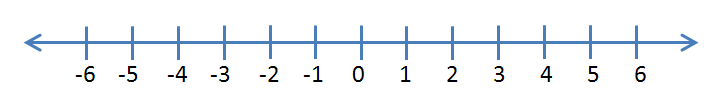
\includegraphics[width=4.5in]{images/integer_line.png}
%\end{center}
%\caption{The usual number line}
%\end{figure}

%But if we replaced each integer in Figure~\ref{fig:integers} with its value (mod 5), then it would look like Figure \ref{integers_mod_5} (we have seen this figure before!):   

%\begin{figure}[h]\label{integers_mod_5}
%\begin{center}
%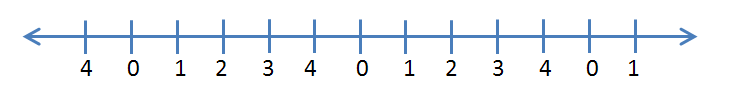
\includegraphics[width=4.5in]{images/integers_mod_5.png}
%\end{center}
%\caption{The number line mod $5$}
%\end{figure}

%The whole infinite set of integers is reduced to repetitive cycles of the integers $0-4$; which is actually what you would expect.  After all, from our modular equivalence section we know 

%\begin{center}
%$... \equiv -10 \equiv -5 \equiv 0 \equiv 5 \equiv 10 \equiv ... \pmod{5}$; \\
 %$... \equiv -9 \equiv -4 \equiv 1 \equiv 6 \equiv 11 \equiv ... \pmod{5}$; \\
  %$... \equiv -8 \equiv -3 \equiv 2 \equiv 7 \equiv 12 \equiv ... \pmod{5}$; \\
  %$... \equiv -7 \equiv -2 \equiv 3 \equiv 8 \equiv 13 \equiv ... \pmod{5}$; \\ 
 %etc. \\  
%\end{center}
%So all the numbers equal to 0 mod 5 are labeled 0; all the numbers equal to 1 mod 5 are labeled 1; and so on.  (In a later chapter you will see that sets of equivalent objects like this are called ``equivalence classes''). We will call this set of 5 labels $\{0,1,2,3,4\}$ the \term{set of integers mod 5}, and denote it by the symbol ${\mathbb Z}_{5}$. 

%In view of this definition, can you see what the set ${\mathbb Z}_{10}$ should be?  How about ${\mathbb Z}_{20}$?  A little thought should convince you that it is natural to choose ${\mathbb Z}_{n} = \{0,1,2,...,n-1\}$.  From our earlier sections we know that you can add and multiply these numbers mod $n$, and obtain a result that is also in ${\mathbb Z}_{n}$.  This motivates the following general definition integers mod $n$: 

%\begin{defn}{}
%Given any positive integer $n$, the set of integers $\{0,1,...,n-1\}$, together with the operations of addition and multiplication mod $n$, are called the \term{integers mod n}.\index{Integers!mod $n$} The symbol ${\mathbb Z}_n$ is used to represent the integers mod $n$.
%\end{defn}
%Later on (in the Equivalence Relations chapter) we'll give the ``correct'' mathematical definition of the integers mod $n$. 


\section{The integers mod $n$ (also known as ${\mathbb Z}_n$)}

\subsection{Arithmetic with remainders}\label{ArithWithRems}
Several times now in this chapter we've simplified our modular calculations by replacing numbers with their remainders mod $n$ (remember, we have defined these remainders as the set ${\mathbb Z}_n$).  We will now fulfill the promise we made at the end of the first section by proving that if you replace numbers with their remainders, we don't change the result of our modular calculations.  That is, we'll show that modular arithmetic can be thought of as \emph{arithmetic with remainders}.

Before we do this, we need to address an important issue. Consider the case of $Z_5 = \{0,1,2,3,4\}$, so 3 and 4 are in $Z_5$. However the sum $3 + 4$ is 7, which is not in $Z_5$. If we're going to do arithmetic with the remainders, we should define a ``sum'' on $Z_n$ such that the result is also in $Z_n$. This motivates the following two definitions:

% We start by introducing two symbols:

% \begin{itemize}
% \item 
% We will use ``$\oplus$" instead of ``$+$" to denote modular addition; that means ``$+$" now strictly means regular addition.
% \item
% We will use ``$\odot$" instead of ``$\cdot$" to denote modular multiplication; that means ``$\cdot$" now strictly means regular multiplication.
% \end{itemize}

% \noindent
% With these in mind, we formally define modular addition and multiplication as follows:

\begin{defn}\label{definition:modular:mod_add}
\term{Modular Addition}\index{Modular addition}

\noindent
The sum mod $n$ of two integers mod $n$ is the remainder left after dividing their regular sum by $n$; that is, if $x,y \in {\mathbb Z}_n$ then

\begin{center}
$x \oplus y = r$ iff  $x + y = r + sn$ and 
$r \in {\mathbb Z}_n.$
\end{center}
\end{defn}
Note that in Definition~\ref{definition:modular:mod_add} we write $x \oplus y = r$ rather than $x \oplus y \equiv r \pmod{n}$, since $x \oplus y$ is defined to be \emph{equal} to the remainder. The same holds for the following definition:

\begin{defn}\label{definition:modular:mod_mult}
\term{Modular Multiplication}

\noindent
The product mod $n$ of two integers mod $n$ is the remainder left after dividing their regular product by $n$; that is, if $x,y \in {\mathbb Z}_n$ then

\begin{center}
$x \odot y = r$ iff  $x \cdot y = r + sn$ and 
$r \in {\mathbb Z}_n.$
\end{center}
\end{defn}
It is important to note that the operations $\oplus$ and $\odot$ \emph{depend on the modulus involved}. We must always make sure that the modulus is clearly specified before talking about $\oplus$ and $\odot$.

Our first step towards showing that ordinary arithmetic can be replaced with arithmetic with remainders is the following proposition:

\begin{prop}{number_remainder}
Given $a,c \in {\mathbb Z}$ and $b,d \in {\mathbb Z_n}$. If $a \equiv b \pmod{n}$ and $c \equiv d \pmod{n}$, then 
\begin{enumerate}[(a)]
\item
$a + c \equiv b \oplus d \pmod{n}$, 
\item
$a \cdot c \equiv b \odot d \pmod{n}$.
\end{enumerate}
\end{prop}

\noindent
We will furnish the proof of part (a): part (b) will be left as an exercise.

\begin{proof}
Since $a \equiv b \pmod{n}$ and $c \equiv d \pmod{n}$, then
\[ a = b + sn \mathrm{~~~and~~~} c = d + tn  \mathrm{~~~~~~(definition~of~modular~equivalence)} \]
Therefore, 
\[ a + c = b + d + (s + t)n \mathrm{~~~~~~(subs.~and~ basic~algebra)} \]
Now by the definition of $\oplus$ there is some $p \in {\mathbb Z}$ such that  $b + d = (b \oplus d) + pn$; therefore 
\[ a + c = (b \oplus d) + pn + (s + t)n = (b \oplus d) + ( p + s + t)n. \mathrm{~~~~~~(subs.~and~ basic~algebra)} \]
Hence by the definition of modular equivalence, 
\[ a + c \equiv b \oplus d \pmod{n}. \]
\end{proof}

\begin{exercise}{44}
\begin{enumerate}[(a)]
\item
Prove part (b) of Proposition~\ref{proposition:modular:number_remainder}.
\item
Come up with a definition for modular subtraction (use the symbol $\ominus$).
\item
Using your definition, prove the following:

\noindent
Given $a,c \in {\mathbb Z}$ and $b,d \in {\mathbb Z_n}$. If $a \equiv b \pmod{n}$ and $c \equiv d \pmod{n}$, then  $a - c \equiv b\ominus d \pmod{n}$.
\end{enumerate}
\end{exercise}

Now that we have proven Proposition~\ref{proposition:modular:number_remainder}, we can combine operations into more complicated equations and show equivalence.

\begin{exercise}{ModPower}
\begin{enumerate}[(a)]
\item
Using part (b) of Proposition~\ref{proposition:modular:number_remainder} above, 
show that if $a \in {\mathbb Z}$ and $b \in {\mathbb Z_n}$ and $a \equiv b \pmod{n}$ then $a^2 \equiv b \odot b \pmod{n}$.
\item 
Using part (a) prove a similar relation involving $a^3$.
\item 
Using part (b) prove a similar relation involving $a^4$.
\item
From parts (a),(b) and (c), what do you conclude about $a^k$ where $k$ is any natural number?
\end{enumerate}
\end{exercise}


\begin{exercise}{ops}
\begin{enumerate}[(a)]
\item
Given $a,c,e \in {\mathbb Z}$ and $b,d ,f \in {\mathbb Z_n}$ where $a \equiv b \pmod{n}$,  $c \equiv d \pmod{n}$, and $e \equiv f \pmod{n}$. Show using Proposition~\ref{proposition:modular:number_remainder} that  
\[ (a + c) + e \equiv (b \oplus d) \oplus f \pmod{n}. \]
\hyperref[sec:modular_arithmetic:hints]{(*Hint*)}
\item
Given $a,c,e \in {\mathbb Z}$ and $b,d ,f \in {\mathbb Z_n}$ where $a \equiv b \pmod{n}$,  $c \equiv d \pmod{n}$, and $e \equiv f \pmod{n}$. Show using Proposition~\ref{proposition:modular:number_remainder} that  
\[ (a \cdot c) + e \equiv (b \odot d) \oplus f \pmod{n}. \]
\item
Given $a,c,e \in {\mathbb Z}$ and $b,d ,f \in {\mathbb Z_n}$ where $a \equiv b \pmod{n}$,  $c \equiv d \pmod{n}$, and $e \equiv f \pmod{n}$. Show using Proposition~\ref{proposition:modular:number_remainder} that  
\[ (a + c) \cdot e \equiv (b \oplus d) \odot f \pmod{n}. \]
\end{enumerate}
\end{exercise}

In the same way as in Exercise~\ref{exercise:modular:ops}, it is possible to show that \emph{any} arithmetical expression involving integers with no matter how many additions, multiplications, and subtractions, can be shown to be equivalent mod $n$ to the corresponding arithmetical expression in ${\mathbb Z}_n$ using the modular operations $\oplus, \odot, \ominus$.

This completes our discussion showing that arithmetic mod $n$ can be reduced to arithmetic in ${\mathbb Z}_n$.  What we've shown can simplify other modular arithmetic arguments as well:

\begin{exercise}{number_remainder}
Prove the following proposition.

\noindent {\bf Proposition}: Given $a,b,c,d \in {\mathbb Z}$ where $a \equiv b \pmod{n}$ and $c \equiv d \pmod{n}$, then 

\begin{enumerate}[(a)]
\item
$a + c \equiv b + d \pmod{n},$ 
\item
$a \cdot c \equiv b \cdot d \pmod{n}$.
\end{enumerate}

Note these are slightly different from (a) and (b) of  Proposition~\ref{proposition:modular:number_remainder} (in fact, to prove (a) here you need to use  part (a) of   Proposition~\ref{proposition:modular:number_remainder} twice, and similarly for (b)).
\end{exercise}

\begin{exercise}{}
Prove or disprove:
\begin{enumerate}[(a)]
\item
$833 \cdot 222 \cdot 949 \equiv 133 \cdot  922 \cdot 249 \pmod{7}$
\item
$(12345 \cdot 6789) + 1357 \equiv (98765 \cdot 13579) + 9876 \pmod{10}$
\end{enumerate}
\end{exercise}


\subsection{Cayley tables for ${\mathbb Z}_n$}
The fact that we can replace integers with their remainders mod $n$ leads us to a simpler way of  thinking about modular arithmetic.  First, recall the integer number line, pictured (again) in Figure~\ref{fig:integers}:
%that when we talked about the car going around a racetrack, the displacements corresponded to
%As we also saw in the racetrack example, 
\begin{figure}[h]
\begin{center}
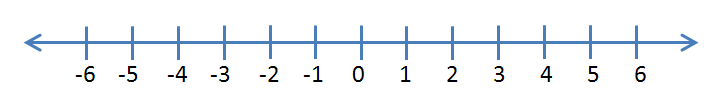
\includegraphics[width=4.5in]{images/integer_line.png}
\end{center}
\caption{The usual number line\label{fig:integers}}
\end{figure}
We may relabel the integers with their remainders mod $5$, pictured in Figure~\ref{fig:integers_mod_5}:
\begin{figure}[h]
\begin{center}
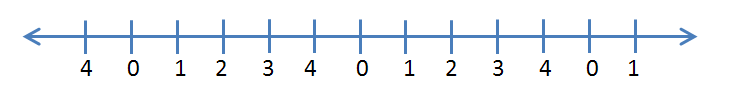
\includegraphics[width=4.5in]{images/integers_mod_5.png}
\end{center}
\caption{The number line mod $5$ \label{fig:integers_mod_5}}
\end{figure}
All the numbers equivalent to 0 mod 5 are labeled 0; all the numbers equivalent to 1 mod 5 are labeled 1; and so on.  The whole infinite set of integers then is reduced to repetitive cycles of the integers $0$ through $4$.  In other words, all the integers are equivalent to either $0, 1, 2, 3,$ or $4$, mod $5$.  

Furthermore, as we just discussed, the sum and product mod $5$ of any two numbers is exactly equivalent to the sum and product mod $5$ of their corresponding remainders.  Therefore, the sum or product of \emph{any} two numbers mod $5$ can be determined by the sum or product of the integers $0-4$.  So we only have to focus on the sums and products of these five numbers to get the result of any modular calculation mod $5$.  

Let's calculate these sums and products then.  We are only using the remainders for mod $5$ (recall we have already defined this set as  ${\mathbb Z}_{5}$).
The following table then gives the results of addition mod $5$ for ${\mathbb Z}_{5}$:

\begin{table}[h]
\caption{\label{groups_Z5_add_table}Addition table for ${\mathbb Z}_5$}{\small
\begin{center}
\begin{tabular}{c|cccccccc}
$\oplus$ & 0 & 1 & 2 & 3 & 4 \\
\hline
0        & 0 & 1 & 2 & 3 & 4 \\
1       & 1 & 2 & 3 & 4 & 0 \\
2       & 2 & 3 & 4 & 0 & 1\\
3       & 3 & 4 & 0 & 1 & 2\\
4       & 4 & 0 & 1 & 2 & 3\\

\end{tabular}
\end{center}
}
\end{table}

\noindent
As an example of how to read this table, the entry in the ``2'' row and the ``3'' column is 0, which tells us that $2 \oplus 3 = 0$ 
(remember, this result depends on fact that we're working in mod 5).

The following table gives the results of multiplication mod $5$ for ${\mathbb Z}_{5}$:

\begin{table}[h]
\caption{\label{groups_Z5_mult_table} Multiplication table for ${\mathbb Z}_5$}
{ \small
\begin{center}
\index{Table!multiplication} 
\begin{tabular}{c|cccccccc}
$\odot$ & 0 & 1 & 2 & 3 & 4 \\
\hline
0       & 0 & 0 & 0 & 0 & 0 \\
1       & 0 & 1 & 2 & 3 & 4  \\
2       & 0 & 2 & 4 & 1 & 3  \\
3       & 0 & 3 & 1 & 4 & 2  \\
4       & 0 & 4 & 3 & 2 & 1  \\

\end{tabular}
\end{center}
}
\end{table}

\noindent
Again, looking at the entry in the ''2'' row and the ''3'' column we see 1, which tells us that $2 \odot 3 = 1$.

Similarly, for each set of numbers ${\mathbb Z}_n$ we can construct a table to determine the result of any possible calculation mod $n$.
These type of tables are known as \term{Cayley tables}\index{Cayley table}.  We will see them often throughout the course.

\begin{exercise}{49}
Use the Cayley table to calculate each of the following using $\oplus$ and $\odot$ in ${\mathbb Z}_5$ (remember, compute the remainders \emph{before} doing the arithmetic).

\begin{enumerate}[(a)]
\item
$ \mod(456 \cdot (252 + 54),5) $
\item
$ \mod(523 + \left( 4568 \cdot (43 + 20525) \right),5)$
\item
$\mod((456 \cdot 252) + (456 \cdot 54),5) $
\item
$ \mod(523 + \left( (4568 \cdot 43) + (4568 \cdot 20525) \right) ,5)$
\end{enumerate}
\end{exercise}

%%% Redundant
% Now imagine relabeling the number line with each integer's remainder mod $10$.  What numbers would be in the set  ${\mathbb Z}_{10}$ then?   What about the set ${\mathbb Z}_{20}$?  What about for ${\mathbb Z}_{n}$? A little thought should convince you that ${\mathbb Z}_{n} = \{0,1,2,...,n-1\}$, since these are all the possible remainders mod $n$.  This motivates the following general definition of the integers mod $n$: 

% \begin{defn}{}
% Given any positive integer $n$, the set of integers $\{0,1,...,n-1\}$ are called the \term{integers mod n}.\index{Integers!mod $n$} The symbol ${\mathbb Z}_n$ is used to represent the integers mod $n$.
% \end{defn}

\noindent
Later on (in the chapter on Equivalence Relations) we'll show another way of looking at the integers mod $n$.

\subsection{Closure properties of ${\mathbb Z}_n$}\label{sec:ClosureZn}

Recall that in Chapter 1 we introduced the complex numbers, then studied their arithmetic properties. In this section, we'll do the same thing with the numbers ${\mathbb Z}_n$ that we have just defined. 

%With ${\mathbb Z}_n$ we have the advantage that the set of numbers is \emph{finite}, so we have can represent the addition and multiplication operations in the form of tables. 

\begin{example}{} 
To start exploring, first consider ${\mathbb Z}_8$. Tables ~\ref{groups_Z8_add_table} and ~\ref{groups_Z8_mult_table} are the addition and multiplication tables for ${\mathbb Z}_8$, respectively.

\begin{table}[h]
\caption{\label{groups_Z8_add_table}Addition table for ${\mathbb Z}_8$}{\small
\begin{center}
\begin{tabular}{c|cccccccc}
$\oplus$ & 0 & 1 & 2 & 3 & 4 & 5 & 6 & 7 \\
\hline
0        & 0 & 1 & 2 & 3 & 4 & 5 & 6 & 7 \\
1       & 1 & 2 & 3 & 4 & 5 & 6 & 7 & 0 \\
2       & 2 & 3 & 4 & 5 & 6 & 7 & 0 & 1\\
3       & 3 & 4 & 5 & 6 & 7 & 0 & 1 & 2\\
4       & 4 & 5 & 6 & 7 & 0 & 1 & 2 & 3\\
5       & 5 & 6 & 7 & 0 & 1 & 2 & 3 & 4\\
6       & 6 & 7 & 0 & 1 & 2 & 3 & 4 & 5\\
7       & 7 & 0 & 1 & 2 & 3 & 4 & 5 & 6\\
\end{tabular}
\end{center}
}
\end{table}

\begin{table}[h]
\caption{\label{groups_Z8_mult_table} Multiplication table for ${\mathbb Z}_8$}
{ \small
\begin{center}
\index{Table!multiplication} 
\begin{tabular}{c|cccccccc}
$\odot$ & 0 & 1 & 2 & 3 & 4 & 5 & 6 & 7 \\
\hline
0       & 0 & 0 & 0 & 0 & 0 & 0 & 0 & 0 \\
1       & 0 & 1 & 2 & 3 & 4 & 5 & 6 & 7 \\
2       & 0 & 2 & 4 & 6 & 0 & 2 & 4 & 6 \\
3       & 0 & 3 & 6 & 1 & 4 & 7 & 2 & 5 \\
4       & 0 & 4 & 0 & 4 & 0 & 4 & 0 & 4 \\
5       & 0 & 5 & 2 & 7 & 4 & 1 & 6 & 3 \\
6       & 0 & 6 & 4 & 2 & 0 & 6 & 4 & 2 \\
7       & 0 & 7 & 6 & 5 & 4 & 3 & 2 & 1
\end{tabular}
\end{center}
}
\end{table}
\end{example}

%\medskip{}
%Recall our definitions of addition and multiplication mod $n$:  For two integers $a$ and $b$, define addition modulo $n$ to be $a + b \pmod{n}$; that is, the remainder when $a + b$ is divided by $n$.  Similarly, multiplication modulo $n$ is defined as $a \cdot b \pmod{ n}$, the remainder when $a  b$ is divided by $n$.

%\medskip{}
There is an important feature exhibited in both Table~\ref{groups_Z8_add_table} and Table ~\ref{groups_Z8_mult_table} that is easy to overlook.
Notice that every entry in the table is also an element of ${\mathbb Z}_8$. You can think of the set $\{0,...,7\}$ as a closed box, and when you add or multiply any two numbers in that box mod $8$, you always get another number in that box, never outside of it (indeed because addition and multiplication mod $8$ return a remainder that is some number $0-7$). We express this mathematically by saying that ${\mathbb Z}_8$ is \term{closed} \index{Closure!integers mod n} under addition and multiplication mod $8$. It seems reasonable that the same should be true for any ${\mathbb Z}_n$, and we state this formally as a proposition (as mathematicians are wont to do):

%While we understand why the entries in the tables below are all integers in ${\mathbb Z}_8$, doesn't it seem a bit fortuitous, even a miracle, that this is true?  How many groups of objects in life can you pick any two out of, combine them in some way, and from that process generate another object in that group, never generating any object outside of it?  You can think of the set $\{0,...,7\}$ as a closed box, and when you add or multiply any two numbers in that box mod $8$, you always get another number in that box, never outside of it.  This fact, this happenstance is a property we call \term{closure} \index{Closure!definition}.  We would say that ${\mathbb Z}_8$ is closed under addition and multiplication mod $8$.

%Now as mentioned above, by the \emph{definitions} of modular addition and multiplication, this closure property should hold not only for ${\mathbb Z}_8$, but for any ${\mathbb Z}_n$.  This motivates our first proposition:

 \begin{prop}{closed_property_Zn}
${\mathbb Z}_n$ is closed under modular addition and multiplication, for all positive integers $n$.
\end{prop}

\begin{exercise}{52}
Prove Proposition~\ref{proposition:modular:closed_property_Zn}. That is, show that the modular sum and modular product of two elements of  ${\mathbb Z}_n$ are also in ${\mathbb Z}_n$.
\hyperref[sec:modular_arithmetic:hints]{(*Hint*)}
\end{exercise}
Please note that closure is not in general a trivial property, and there are many examples of number systems that are not closed under various operations. For instance, the positive integers are not closed under the operation of subtraction, because (for example) $5 - 7$ is not a positive integer. Similarly, the positive integers are not closed under the operation of square root, because the square root of 2 is not an integer.

\begin{exercise}{53}
For each of the following number systems, indicate whether or not they are closed under (i) addition (ii) subtraction (iii) multiplication (iv) division (v) square root.
\hyperref[sec:modular_arithmetic:hints]{(*Hint*)}  
\begin{multicols}{2}
\begin{enumerate}[(a)]
\item
The integers 
\item
The rational numbers
\item
The real numbers
\item
The positive rational numbers
\item
The positive real numbers
\item
The nonzero real numbers
\end{enumerate}
\end{multicols}
\end{exercise}

\begin{exercise}{54}
Prove that the complex numbers are closed under complex addition and multiplication.
\end{exercise}

\subsection{Identities and inverses in ${\mathbb Z}_n$}
Next, we want to look at some additional properties that were introduced in Chapter~\ref{complex}, namely 
 identities  and inverses (both additive and multiplicative).  
This time we'll go through these properties more quickly.

Do the integers mod $n$ have an additive identity for all $n$?  In other words, is there a specific integer mod $n$ that added to $a$ leaves $a$ unchanged? For the specific case of ${\mathbb Z}_8$, we can see from the first row of Table~\ref{groups_Z8_add_table} that 
$0 \oplus a = a $ for any $a \in {\mathbb Z}_8$. Similarly, the first column of Table~\ref{groups_Z8_add_table} show that $a \oplus 0 = a$ for any $a \in {\mathbb Z}_8$. Is this true for \emph{any} ${\mathbb Z}_n$? the following proposition shows that it is. 
\index{Integers mod n!additive identity}
% From our definition of modular addition (ordinary addition followed by taking the remainder), it should be clear that the same will be true for any ${\mathbb Z}_n$. It follows that plus (any number in ${\mathbb Z}_8$) Similarly, is there a specific integer mod $n$ that when you multiply it by any other integer $a \pmod{n}$, you get $a$?  From your knowledge of integers you can probably guess that the additive identity is $0$, while the multiplicative identity is $1$, which are in ${\mathbb Z}_n \forall n$.  And if you look at the addition and multiplication Tables for ${\mathbb Z}_8$ in the previous section, you can see an example of this.  In every row of the addition table, the spot under the $0$ column contains the row number; and in every row of the multiplication table, the spot under the $1$ column contains the row number.  Therefore:


\begin{prop}{id_property_Zn}
$0 \in {\mathbb Z}_n$ is the additive identity of ${\mathbb Z}_n$.
\end{prop}
\begin{proof} Given any $a \in {\mathbb Z}_n$, then $a \oplus 0$ is computed by (a) compute $a + 0$ using ordinary addition, then (b) taking the remainder mod $n$. Since $a + 0 = a$, and $0 \leq a < n$, it follows that the remainder is also $a$. Hence $a \oplus 0 = a $. We can show that $0 \oplus a = a $ in the same way. Thus $0$ satisfies the definition of identity for ${\mathbb Z}_n$.
\end{proof}

\begin{exercise}{56}
Give a similar proof that $1$ is the multiplicative identity for ${\mathbb Z}_n$ when $n >1$. What is the multiplicative identity for ${\mathbb Z}_n$ when $n=1$?
\end{exercise}


% 0 and multiplicative identity 1, that is:  
% \begin{enumerate}[(a)]
% \item
% $a + 0  &\equiv  0 + a \equiv  a \pmod{ n}$
% \item
% $a \cdot  1  &\equiv  1 \cdot a \equiv  a \pmod{ n}$.
% \end{enumerate} 
% \end{prop}

% Let's prove (a).  

% \begin{exercise}{}
% Fill in the blanks of the following proof:

% \noindent
% Given that $a \in {\mathbb Z}_n$, it follows that
% \begin{enumerate}[(a)]
% \item $a+0 = 0 + \_\_\_ = \_\_\_$ (usual arithmetic), and
% \item $a  \equiv \_\_\_$  (by division algorithm, since $a \in {\mathbb Z}_n$).
% \item Therefore $\_\_\_\_\_\_\_\_\_\_ \equiv \_\_\_\_\_\_\_\_\_\_ \equiv a$ (by the definition of modular equivalence).
% \end{enumerate}
% \end{exercise}

% \begin{exercise}{}
% Give a similar proof to prove the multiplicative portion of Proposition~\ref{proposition:modular:id_property_Zn}.
% \end{exercise}

\subsection{Inverses in ${\mathbb Z}_n$}

Now let's look to see if the integers mod $n$ have additive and multiplicative inverses\index{Inverse!integers mod n}.  For each element of  ${\mathbb Z}_n$ is there a corresponding element of ${\mathbb Z}_8$ such that their modular sum is the additive identity (that is, 0)?  You may see in Table~\ref{groups_Z8_add_table} that each row of the addition table contains the additive identity, $0$ (for example, $1\oplus 7 = 0$).  It follows that in ${\mathbb Z}_8$, each element has an additive inverse.  If we shrink or expand the table to cover all moduli $n$, would we find the same thing in every table?  We should. This motivates the following:

\begin{prop}{addinv_property_Zn}
Let ${\mathbb Z}_n$ be the  integers mod $n$ and $a \in {\mathbb Z}_n$. Then for every  $a$  there is an additive inverse $a' \in {\mathbb Z}_n$.  

In other words: for any $a \in {\mathbb Z}_n$ in  we can find an $a'$ such that:
\[
a \oplus a' = a' \oplus a  = 0.
\]
We structure the proof of Proposition~\ref{proposition:modular:addinv_property_Zn} as an exercise. We prove the two cases $a=0$ and $a \neq 0$ separately.

\begin{exercise}{58}

\begin{enumerate}[(a)]
\item
Show that  $0 \in {\mathbb Z}_n$ has an additive inverse in ${\mathbb Z}_n$.

\item
Suppose $a$ is a nonzero element of ${\mathbb Z}_n$  (in mathematical shorthand, we write this as: $a \in {\mathbb Z}_n \setminus \{0\}$), and let $a' = n-a$.
\begin{enumerate}[(i)]
\item
Show that $a'$ is in ${\mathbb Z}_n$ .
\hyperref[sec:modular_arithmetic:hints]{(*Hint*)}
\item
Show that $a \oplus a' = a' \oplus a  = 0 \pmod{ n}$: that is, $a'$ is the additive inverse of $a$.
\end{enumerate}
\end{enumerate}
\end{exercise}
\end{prop}

Now can we do the same thing for multiplication? That is, for all integers $a$ mod $n$, is there a corresponding integer mod $n$ such that their product is the multiplicative identity?  

Let's see if this is true in ${\mathbb Z}_8$. Consider the multiplication table for ${\mathbb Z}_8$ in Table~\ref{groups_Z8_mult_table}.  Scanning the rows do we find the multiplicative identity $1$ in every row?   

Looking at the table, we find that  rows 0, 2, 4, and 6 do not contain a $1$. We would state this formally in the following way:  for $n = 0$, 2,  4, or 6, there is no integer $k \in {\mathbb Z}_8$ such that $k \odot n \equiv 1 \pmod{ 8}$.  Hence not every integer mod 8 has a multiplicative inverse. 

A little thought should convince you that 0 \emph{never} has a multiplicative inverse for any ${\mathbb Z}_n$. This means that it's not possible to prove a multiplicative version of Proposition \ref{proposition:modular:addinv_property_Zn}, since we have a \term{counterexample} that shows that not every element of ${\mathbb Z}_n$ has an inverse, no matter what $n$ is.

\begin{rem}
This example shows that it's often easier to \emph{disprove} something than to prove it!  To disprove a general statement, you only need to find \emph{just one} counterexample, whereas an unlimited number of examples can never prove a general statement.
\end{rem}

However, all is not lost as far as multiplicative inverses are concerned. We will see later that they play a very important role when we consider arithmetic with the \emph{nonzero} elements of ${\mathbb Z}_n$:

\begin{exercise}{60}
\begin{enumerate}[(a)]
\item
Find an integer $n>2$ such that all \emph{nonzero} elements of ${\mathbb Z}_n$ have multiplicative inverses.
\item
Find two additional values of $n>5$ such that all nonzero elements of ${\mathbb Z}_n$ have multiplicative inverses.
\item
What do the three numbers you found in (a) and (b) have in common?
\end{enumerate}
\end{exercise}

\subsection{Other arithmetic properties of $\oplus$ and $\odot$}

In many respects, $\oplus$ and $\odot$ are very similar to the ordinary arithmetic operations $+$ and $\cdot$. It makes sense that they too should be associative, distributive, and commutative  (recall these properties were defined   in Section~\ref{OpsAndRels}). But as mathematicians, it's not enough for something to ``make sense''. We need solid proof. So, voil\`a:

\begin{prop}{Zn_comm_assoc}
In the following $n$ is an arbitrary positive integer and $a, b, c$ denote arbitrary elements of ${\mathbb Z}_n$.
\begin{enumerate}
 
\item \label{comm} \it %1
Modular addition and multiplication are commutative:\index{Commutative property!modular addition/multiplication}  
\begin{align*}
a \oplus b  & =  b \oplus a  \\
a \odot b   & =  b \odot a .
\end{align*}
 
\item \label{assoc} \it %2
Modular addition and multiplication are associative: \index{Associative property!modular addition/multiplication}
\begin{align*}
(a \oplus b) \oplus c  =  a \oplus (b \oplus c) \\
(a \odot b) \odot c    =  a \odot (b \odot c).
\end{align*}
 
\item \label{distrib} \it %3
Modular multiplication distributes over modular addition: \index{Distributive property!modular addition/multiplication}
\[
a \odot (b \oplus c)  = (a \odot b)\oplus (a \odot c).
\]
\end{enumerate}
\end{prop}

\begin{proof}
We'll do the proof that modular addition is associative, and  you will prove the other statements as exercises (the proofs are pretty similar). The proof strategy is a familiar one: prove modular arithmetic properties by making use of the corresponding properties of ordinary arithmetic.


\term{Modular addition is associative:}
Given $a,b,c$ are elements of $\mathbb{Z}_n$, it's also true that $a,b,c$ are integers. By Proposition~\ref{proposition:modular:number_remainder}, it follows that:
\[ a \oplus b \equiv a + b \pmod{n}. \]
We may use Proposition~\ref{proposition:modular:number_remainder} a second time to obtain:
\[ (a \oplus b) \oplus c  \equiv (a + b) + c \pmod{n}. \]
Using the same reasoning (applying Proposition~\ref{proposition:modular:number_remainder} twice), we can also show that:
\[  a \oplus (b \oplus c)  \equiv a + (b + c) \pmod{n}.\]
Now here's where we use regular arithmetic. The associative property of integer addition tells us that $a + (b + c) = (a+b)+c$,
and we can substitute into the previous equivalence to obtain:
\[a \oplus (b \oplus c)  \equiv (a + b) + c \pmod{n}. \]
We now have two different expressions (namely, $(a \oplus b) \oplus c$ and $a \oplus (b \oplus c)$ that are both equivalent to $(a + b) + c$. So we can apply
Proposition~\ref{proposition:modular:equivalence_transitive} (the ``transitive property'') to get that
\[ (a \oplus b) \oplus c  \equiv  a \oplus (b \oplus c) \pmod{n}. \]
Since  $(a \oplus b) \oplus c$  and  $a \oplus (b \oplus c)$ are both in ${\mathbb{Z}}_n$, it follows from Proposition~\ref{proposition:modular:equiv_mod_n} that  
$(a \oplus b) \oplus c = a \oplus (b \oplus c)$, and the proof is complete. 
\end{proof}
 
\begin{exercise}{}
\begin{enumerate}[(a)]
\item
Prove that addition mod $n$ is commutative.
\item
Prove that multiplication mod $n$ is commutative.
\item
Prove that multiplication mod $n$ is associative.
\item
Prove  part (\ref{distrib}) of Proposition \ref{proposition:modular:Zn_comm_assoc}.
\end{enumerate}
\end{exercise} 

\subsection{Definition of a group}\label{DefOfGroup}
It's time for us to make a confession. All this time we've been talking about modular arithmetic, we've had an ulterior motive. We're not so interested in modular arithmetic for its own sake:\footnote{Although you have to admit it \emph{is} interesting.} rather, we've spent all this time and effort discussing modular arithmetic because it provides good examples of the central concept in abstract algebra, namely, the concept of a \emph{group}.

Notice that the set ${\mathbb Z}_n$ with the operation of $\oplus$ has an identity, and inverses, and the property of closure. Furthermore, ${\mathbb Z}_n$ is associative under $\oplus$, as we just showed.  Any combination of a set and an operation that has those three properties, as well as the associative property, is called a \term{group} \index{Group!definition}

\begin{defn}  A \term{group}\index{Group!definition} is a set combined with an operation that has the following properties:
\begin{itemize}
\item \emph{Closure}: the set is closed under the operation;
\item \emph{Identity}: the set has an identity element for the operation;
\item \emph{Inverse}: every element of the set has an inverse under the operation;
\item \emph{Associative}: the operation is associative.
\end{itemize}
\end{defn}

\noindent
Notice that we do  \emph{not} include the commutative property in this list. Later on we'll see examples of groups that are \emph{not} commutative. 

We have shown that  ${\mathbb Z}_n$ is a group under the operation $\oplus$ for \emph{any} integer $n$. What about multiplication? The answer isn't quite so easy.

\begin{exercise}{64}
\begin{enumerate}[(a)]
\item Show that for $n \ge 2$, ${\mathbb Z}_n$ is \emph{not} a group under $\odot$. 
\hyperref[sec:modular_arithmetic:hints]{(*Hint*)}
\item
Show that the nonzero elements of ${\mathbb Z}_3$ (that is, ${\mathbb Z}_3 \setminus \{0\}$)  is a group under $\odot$.
Is ${\mathbb Z}_n \setminus \{0\}$ a group under $\odot$ for \emph{every} integer $n \ge 2$?  \emph{Justify} your answer.
\end{enumerate}
\end{exercise}


 \section{Modular division}\label{euclidean}

 Before we get to modular division, we'll first look at some preliminary stuff. This all may seem irrelevant, but  please be patient: we'll get to the point soon enough.
 
 
\subsection{A sticky problem}
The following problem may not seem to have anything to do with modular arithmetic, but it's an interesting problem and fun to think about. (And it will also turn out to be relevant after all!)\footnote{This section is by David Weathers (edited by CT).}

\begin{example}{2sticks} Someone gives us a pencil and two unmarked sticks of lengths 52 cm and  20 cm respectively (see Figure~\ref{fig:1euclidean}). We are told to make measuring sticks by using the pencil to make markings on the sticks. Question: what is the smallest length that we can accurately measure? 
\begin{figure}
\begin {center} 
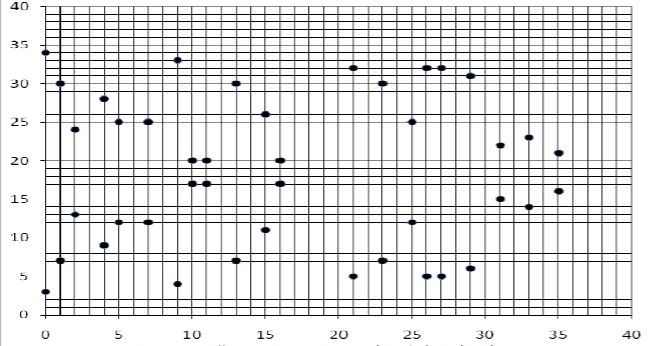
\includegraphics[width=1.00\textwidth]{images/2_sticks_step1.png}
\end {center}
\caption{Two sticks\label{fig:1euclidean}}
\end{figure}
Clearly we can measure 20 cm lengths with the shorter rod, but is it possible to make smaller measurements?

Here's one way to look at the situation. Imagine for a moment that we lay the 20 cm measuring stick next to the 52 cm stick such that the ends line up.  At that point we could make a 20 cm mark on the 52 cm stick (see Figure~\ref{fig:2}).
\begin{figure}
\begin {center} 
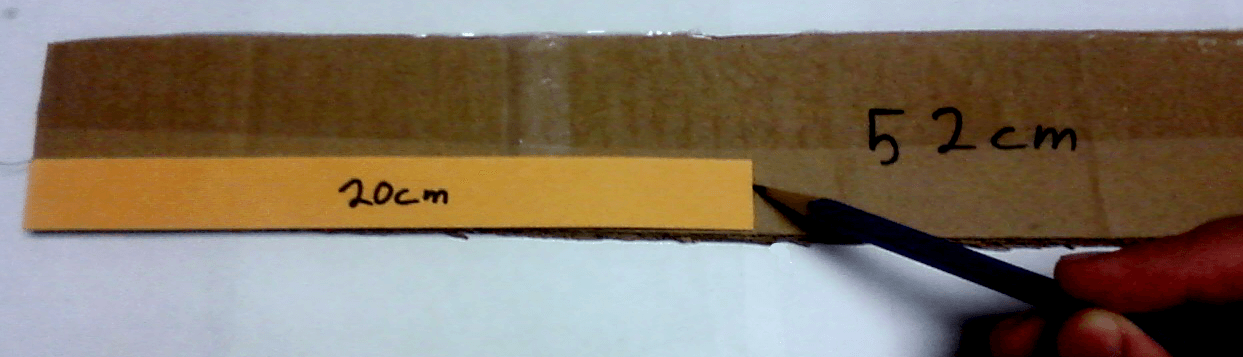
\includegraphics[width=1.00\textwidth]{images/2_sticks_step2.png}
\end {center}
\caption{First mark\label{fig:2}}
\end{figure}

\noindent At this point we move the 20 cm stick further down the the 52 cm stick such that one end is on the pencil mark, and and make another mark.  Now there are two 20 cm sections marked on the 52 cm stick, 
as shown in Figure~\ref{fig:3}.  
\begin{figure}
\begin{center}
	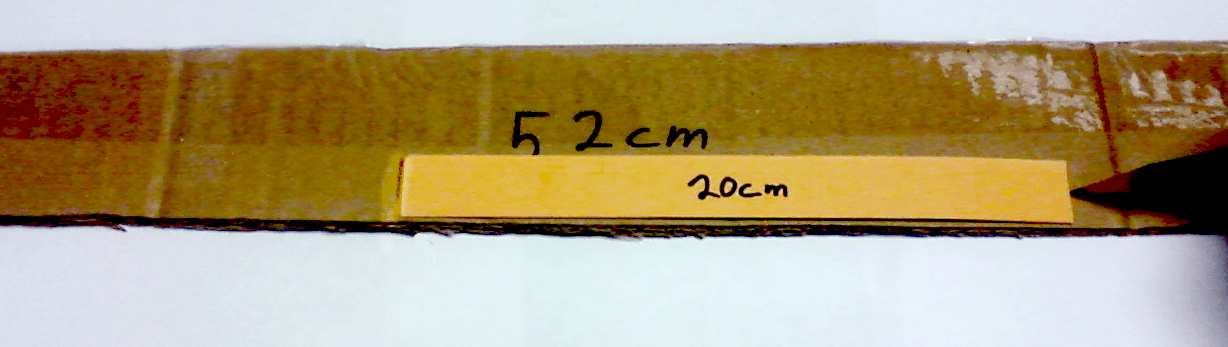
\includegraphics[width=1.00\textwidth]{images/2_sticks_step3.png}
\end{center}
\caption{Second mark\label{fig:3}}
\end{figure}

Since we know the sum of the marked sections is 40 cm, and the length of the large stick is 52 cm, the remainder of the distance must be 12 cm, as shown in Figure~\ref{fig:4}. So we've actually made progress. At the beginning we were only able to measure lengths larger than 20 cm: but now we can measure 12 cm with the latest mark we've made.
\begin{figure}
\begin{center}
	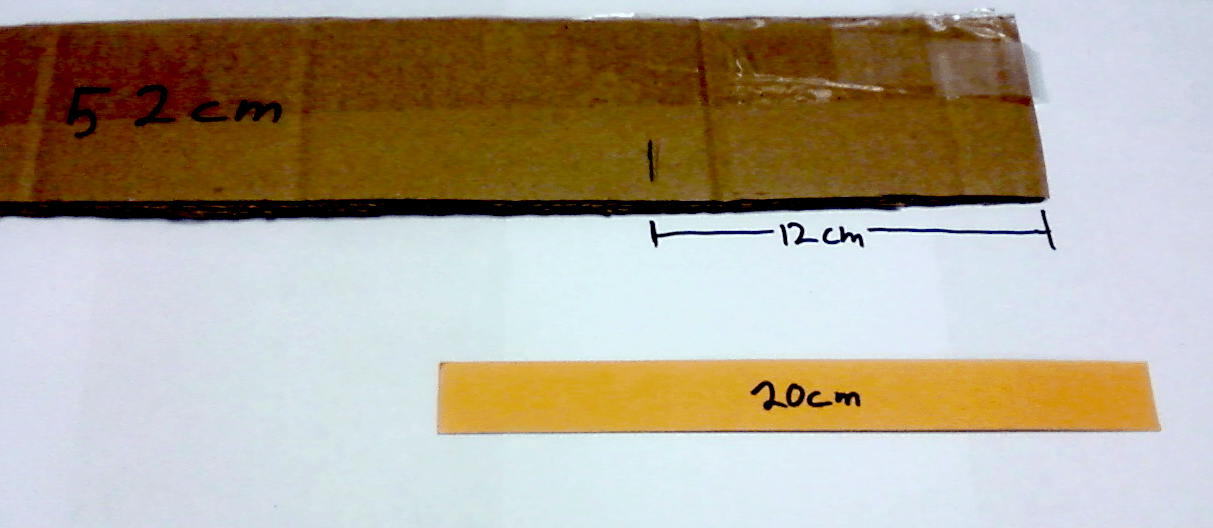
\includegraphics[width=1.00\textwidth]{images/2_sticks_step5.png}
\end{center}
\caption{Remaining distance\label{fig:4}}
\end{figure}

But let's not stop there. We can use the 12 cm section to divide up the 20cm stick. This will subdivide the 20 cm stick into a 12 cm section and a 8 cm section, as shown in Figure~\ref{fig:5}.
\begin{figure}
\begin{center}
	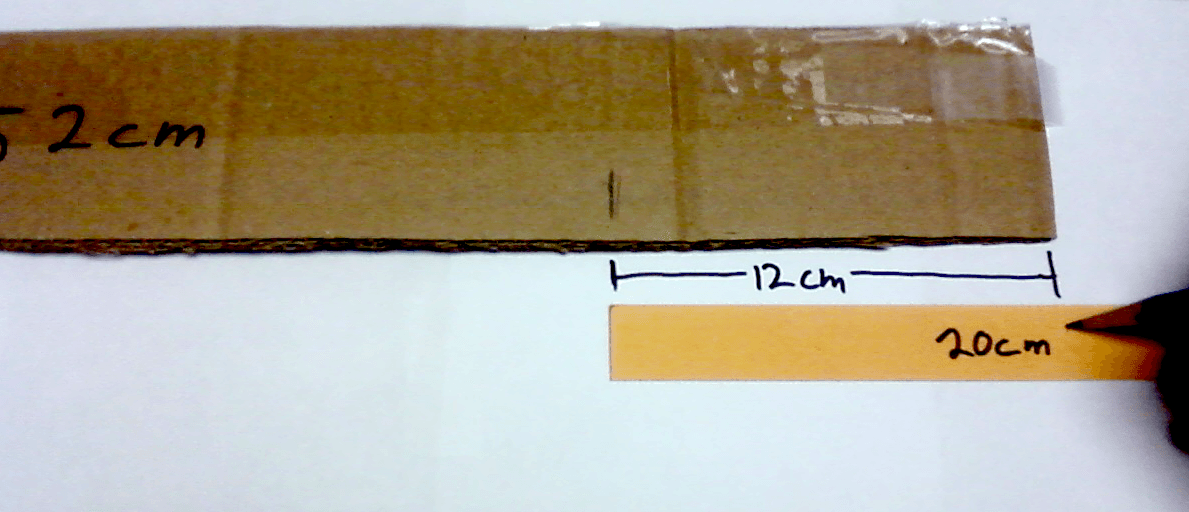
\includegraphics[width=.4900\textwidth]{images/2_sticks_step6.png} 
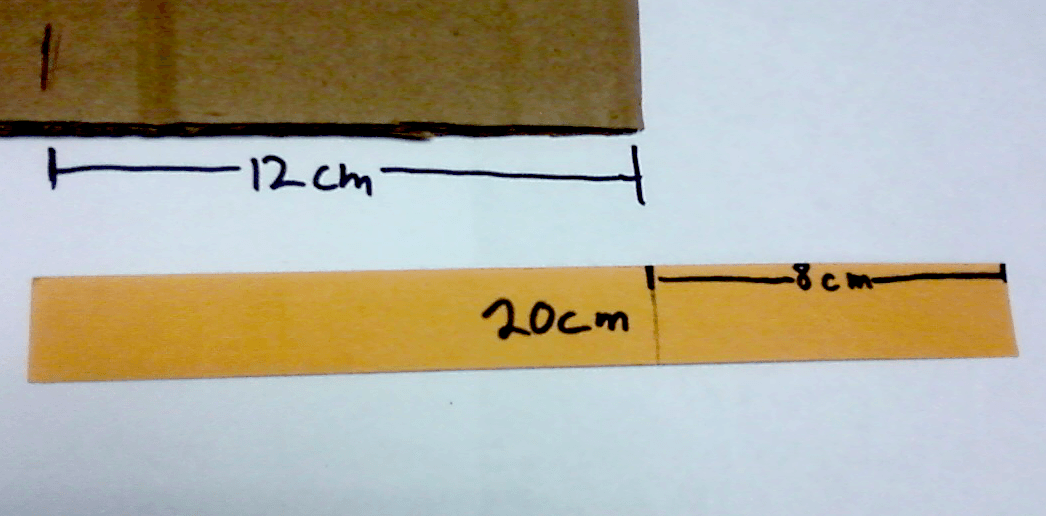
\includegraphics[width=.4900\textwidth]{images/2_sticks_step7.png}
\end{center}
\caption{More subdivision\label{fig:5}}
\end{figure}

Now we're rolling! Let's subdivide the 12 cm section using the 8 cm section.  This will produce an 8 cm section and a 4 cm section (see Figure~\ref{fig:8}).
\begin{figure}
\begin{center}
	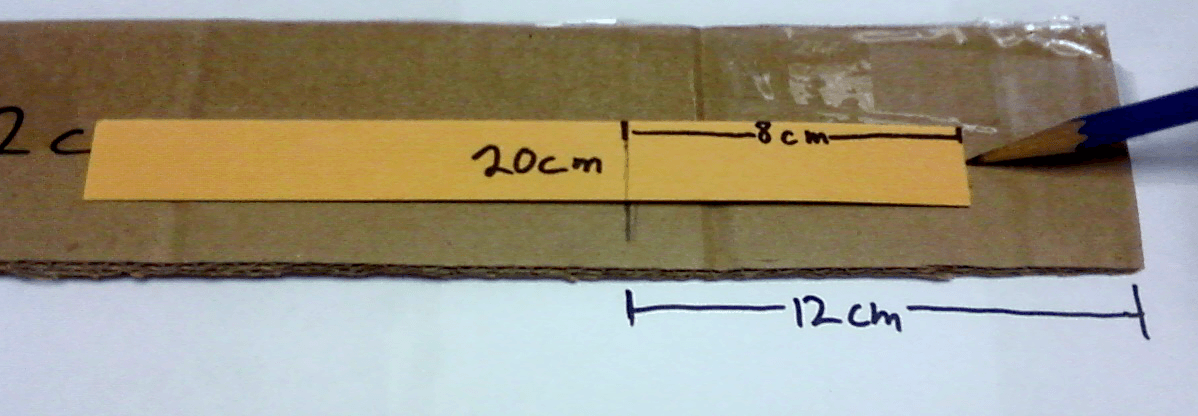
\includegraphics[width=.4900\textwidth]{images/2_sticks_step8.png} 
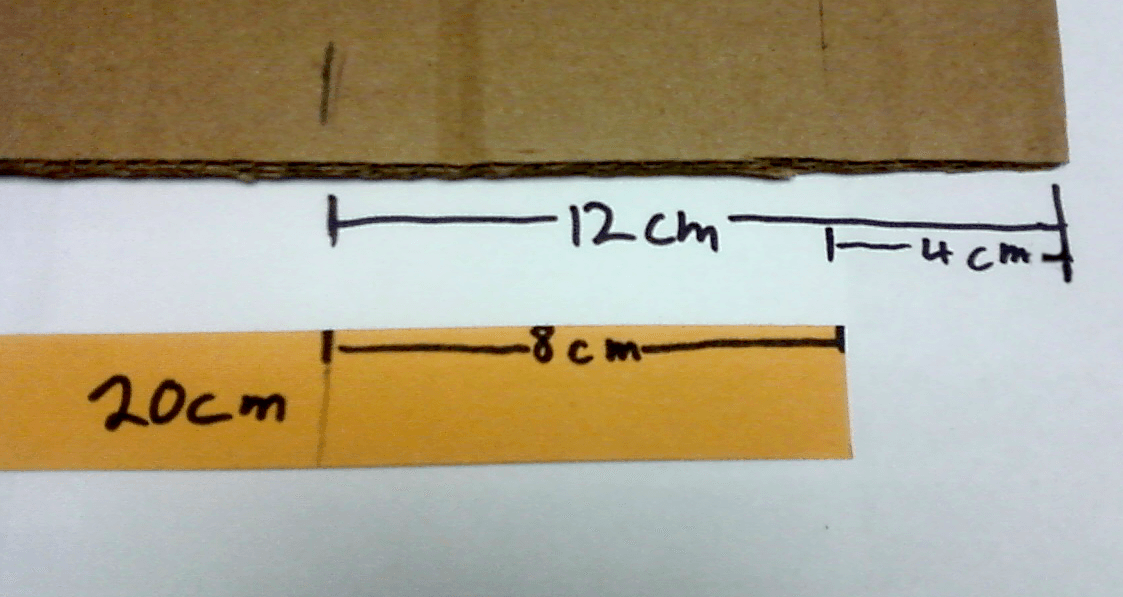
\includegraphics[width=.4900\textwidth]{images/2_sticks_step9.png}
\end{center}
\caption{More subdivision\label{fig:8}}
\end{figure}
Now if we try to use the 4 cm section to subdivide any of the other sections, we will no longer have a remainder.  This is because 4 cm evenly divides all the other lengths we have created, as shown in  Figure~\ref{fig:9}.
\begin{figure}
\begin{center}
	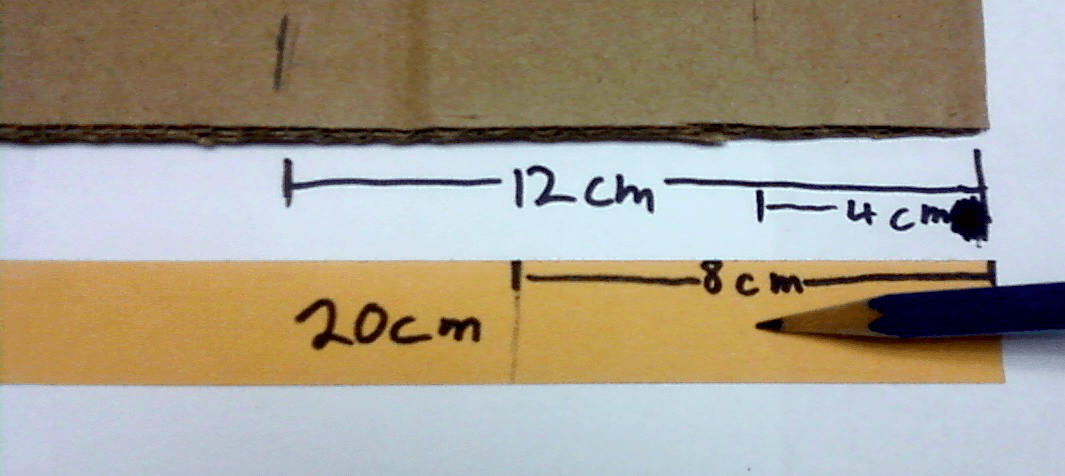
\includegraphics[width=.4900\textwidth]{images/2_sticks_step10.png} 
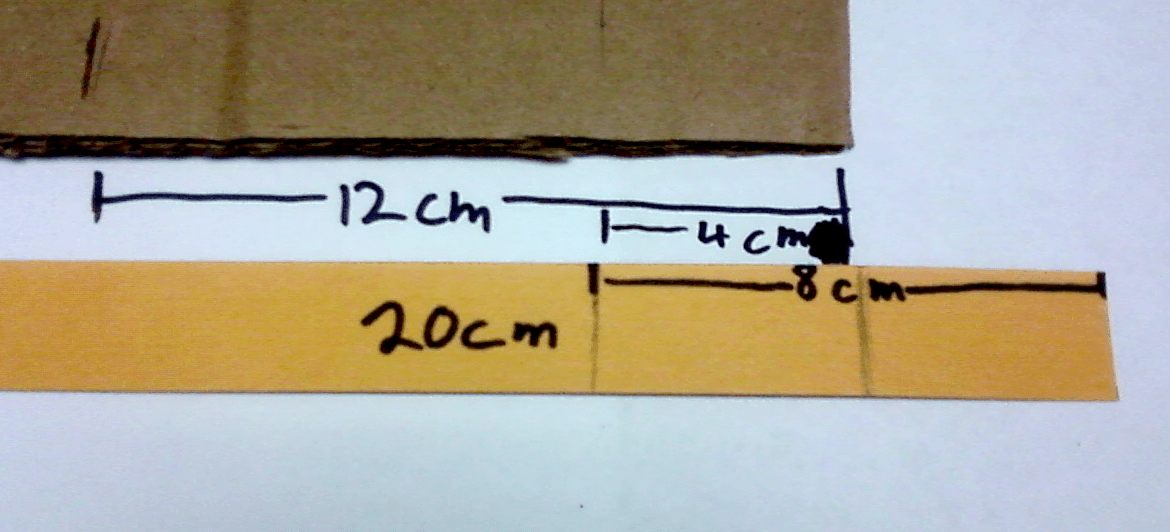
\includegraphics[width=.4900\textwidth]{images/2_sticks_step11.png}

	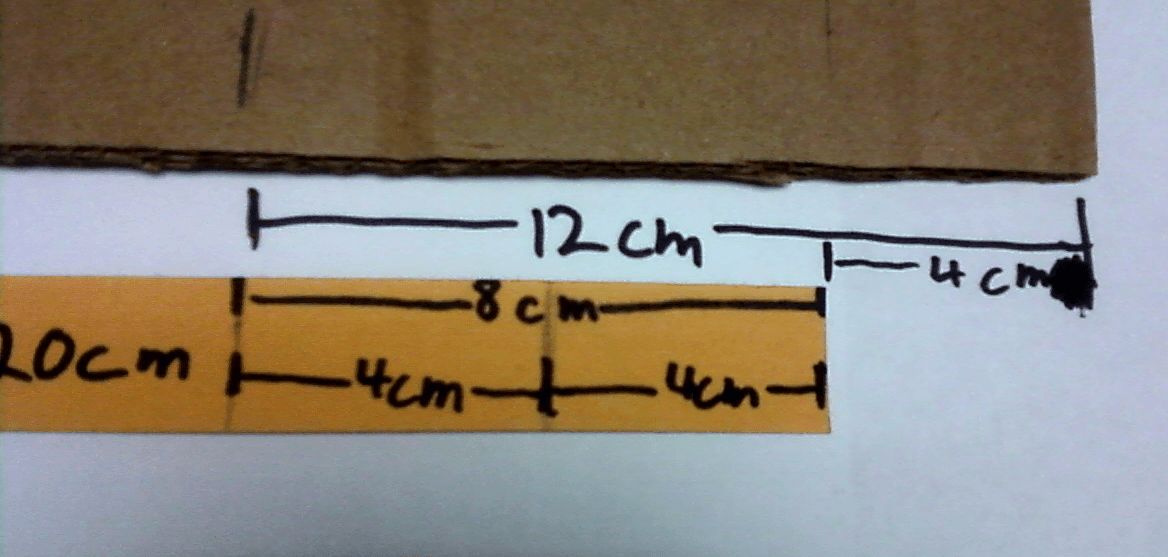
\includegraphics[width=.4900\textwidth]{images/2_sticks_step12.png} 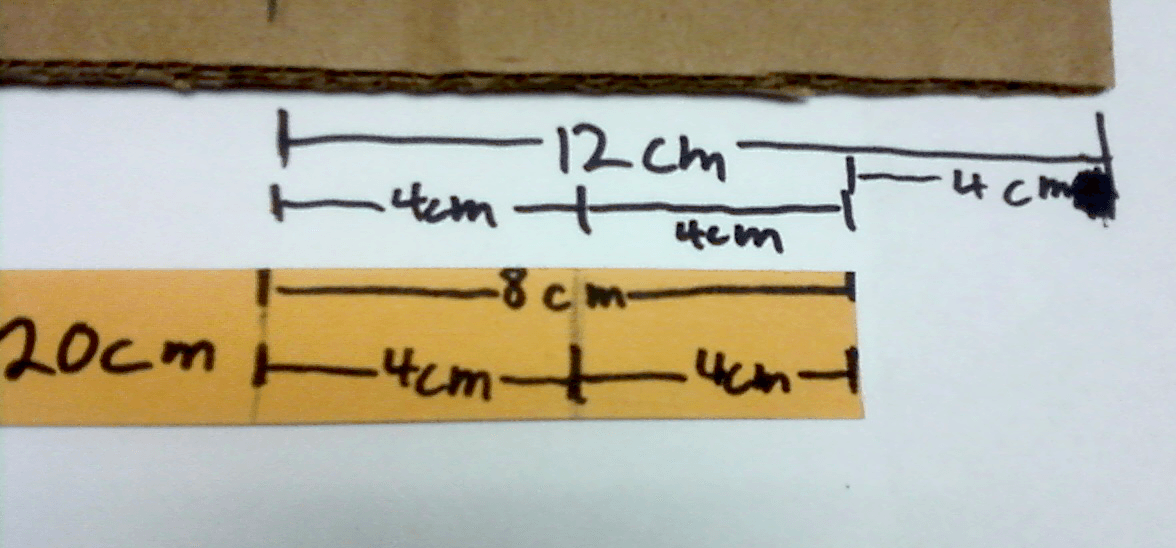
\includegraphics[width=.4900\textwidth]{images/2_sticks_step13.png}

	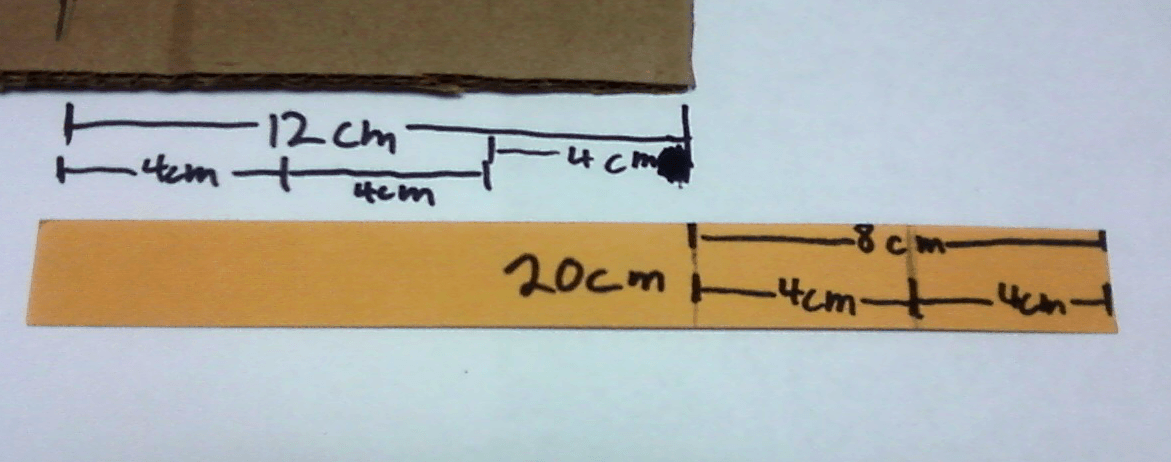
\includegraphics[width=.4900\textwidth]{images/2_sticks_step14.png} 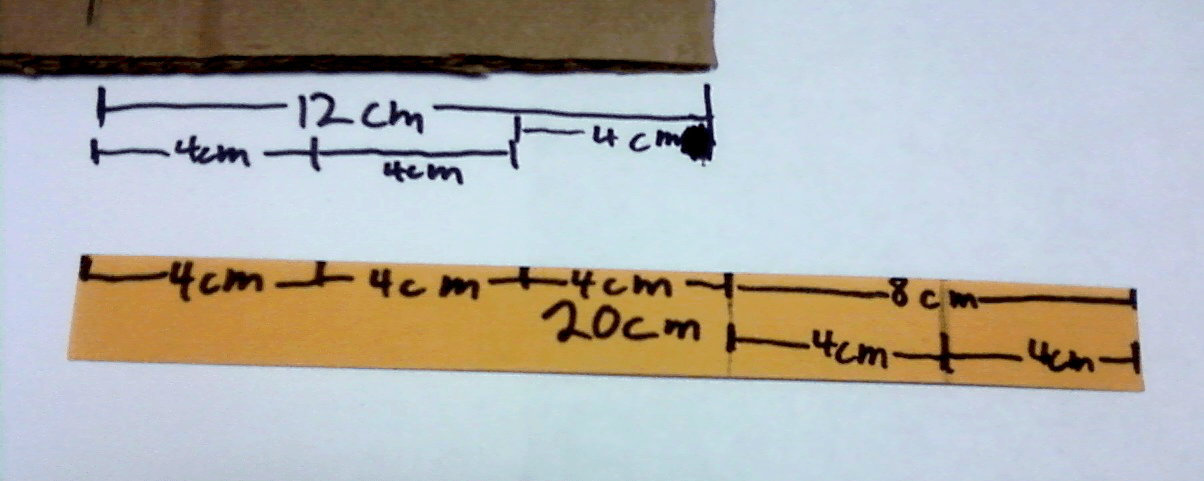
\includegraphics[width=.4900\textwidth]{images/2_sticks_step15.png}

	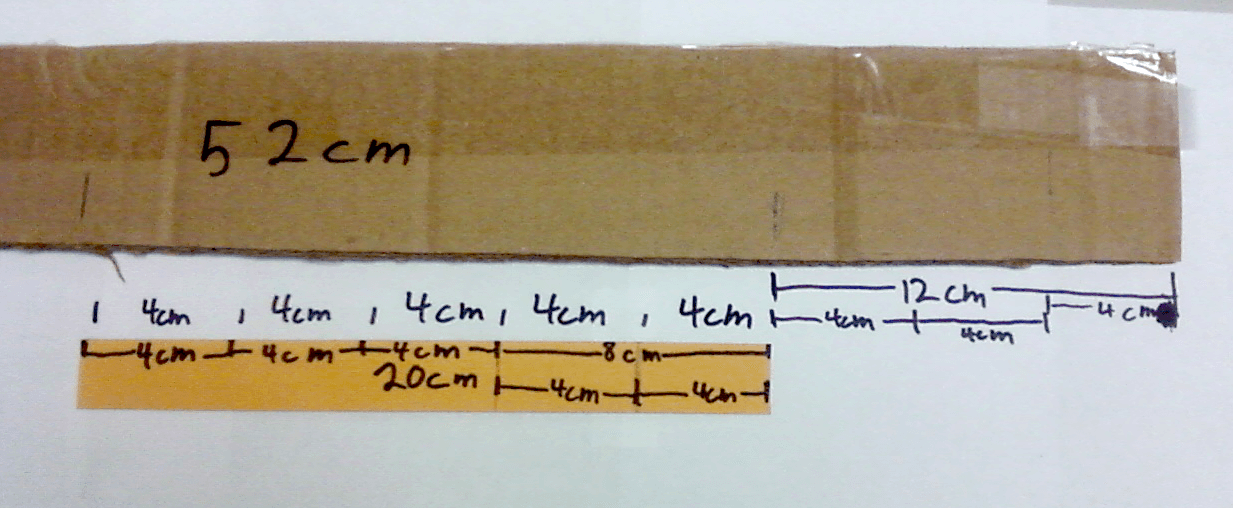
\includegraphics[width=.4900\textwidth]{images/2_sticks_step16.png} 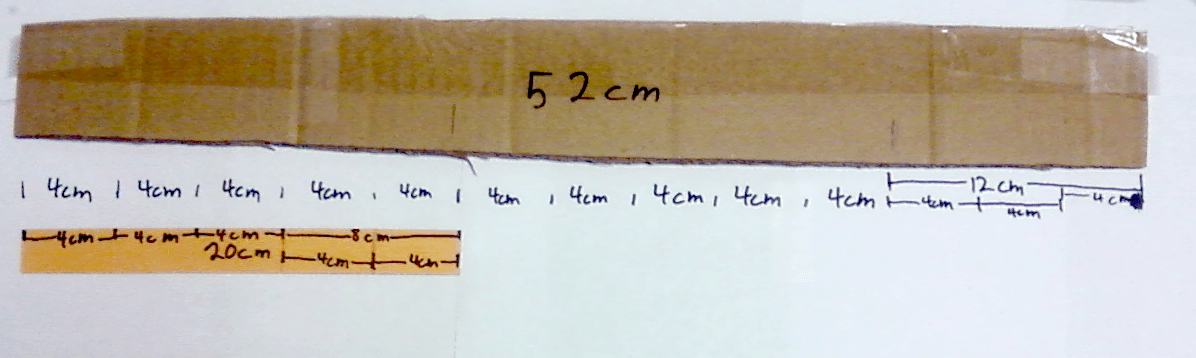
\includegraphics[width=.4900\textwidth]{images/2_sticks_step17.png}
	
\end{center}
\caption{More subdivision\label{fig:9}}
\end{figure}
%So it is proven that 4 cm evenly divides all intervals marked along the way, but is it the only divisor?  Both 52 and 20 are even numbers, which means they are divisible by 2.  But notice, that 4 is also divisible by 2.  This makes an important implication that will be proven later in this chapter.

\end{example}

\begin{exercise}{stick_units}
Using the method above, find the smallest measure given sticks of length:
\begin{enumerate}[(a)]
\item
30 cm and 77 cm.
\item
7 feet and 41 feet (Pretty long sticks!).
\item
33 in and 72 in.
\end{enumerate}
\end{exercise} 


While working on the exercises, you may have noticed that the units of measure used do not matter.  The only thing that matters is the actual count of those units of measure.  

\begin{exercise}{}
Using the method above:
\begin{enumerate}[(a)]
\item
Convert the measurements in Exercise~\ref{exercise:modular:stick_units} part (a) into millimeters, and solve the problem again. How is your result using millimeters related to your answer to part (a) in the previous exercise?
\item
Convert the measurements in Exercise~\ref{exercise:modular:stick_units} part (b) into inches, and solve the problem again. How is your result using inches related to your answer to part (a) in the previous exercise?
\item
Use what you've discovered in part (b) to quickly find a solution to the two-sticks problem when one stick is 720 inches and the other is 600 inches.
\end{enumerate}
\end{exercise}

\subsection{Greatest common divisors}
You may be  familiar with the notion of greatest common divisor (gcd) of two numbers.  The gcd is defined as the greatest number that divides the two given numbers. gcd's play a key role in modular arithmetic, as we shall see. 

The general question we now consider is: What's a good way to find the gcd of two integer numbers? It may be easy to find the gcd of small numbers like 12 and 20, but what if you have to find the gcd of 583768 and 260568447? 

At this point, let's think back to our two-sticks problem. We saw that when we began with sticks of length 52 and 20, we ended up with a minimum measurable distance of 4--which just so happens to be the gcd of 52 and 20! So to get the gcd of 583768 and 260568447, in theory we could try creating one stick of length 583768 and another of length 260568447 and follow the same procedure. Of course this isn't practical. So instead, we'll try to duplicate the same procedure using just algebra, without actually creating the sticks.  Notice that when we subdivided a larger stick of length $a$ into sections of the length of $b$, the result was essentially the same as dividing $a$ by $b$ while leaving a remainder $r$.  See if you can complete the connection in the following example.

\begin {example} {Greatest Common Divisor}
Let's use algebraic language to express the two-sticks algorithm applied to 52 and 20.
Let's start by setting this up as a division problem with a remainder, again since this is effectively what is being done in the stick example above.
\[ 52 = 20\cdot x + b\]

By division with remainder we find $x=2$ and $b=12$
Now we set up the problem again, this time dividing 12 into 20. 

\[ 20 = 12\cdot x + b\]

This yields $x=1, b=8$.  Then set up the problem again, this time dividing 8 into 12.

\[ 12 = 8\cdot x + b\]

This yields $x=1, b=4$.  Then set up the problem again, this time dividing 4 into 8.

\[ 8 = 4\cdot x + b\]

This yields $x=2, b=0$.  

Now notice that 8 is divisible by 4.  In the equation before that, we have $12 = 4\cdot2 + 4$.  Since the right hand side is a sum of multiples of 4, the left hand side must also be a multiple of 4.  In the next equation up $20=12\cdot x + 8$ again, the right hand side is a sum of multiples of 4, so the left hand side must also be a multiple of 4.  Continuing this logic upward shows that all intervals created along the way are divisible by 4.  Hence the algorithm has generated a divisor of the original lengths 52 and 20.  

The procedure we have just described is called the \term{Euclidean algorithm}.\index{Euclidean algorithm}(An \emph{algorithm} is a mathematical procedure designed to compute a specific result). The Euclidean algorithm is very powerful, and in fact can be used to calculate gcd's of large numbers as we'll see below.

 In the above example,  by factoring 52 and 20 into primes: $20=2\cdot2\cdot5$ and $52=2\cdot2\cdot13$, it is plain to see that the only common factors are 2 and 4.  Thus the divisor produced by the Euclidean algorithm happened to be the greatest common divisor. This turns out to be true in general, as we will now prove.

 %%% CPT this is an orphan comment. It doesn't lead anywhere.
%While it is possible to select the divisor and remainder differntly to more quickly arrive at the answer, it becomes a trial %and error process.  However, by simply following the algorithm, one will eventually arrive at a common divisor and that divisor will be the largest.
\end{example}

\begin{prop}{Greatest Common Divisor}
The Euclidean algorithm applied to two integers will give the gcd of those two integers.
\end{prop}
\begin{proof}
This proof is broken up into two parts, (A) and (B).  Part (A) shows that the algorithm always produces a divisor of the two given integers.  Part (B) shows that the produced divisor is indeed the gcd.

\begin {enumerate}[(A)]
\item
Given integers $a$ and $b$ and $a>b$ if we were to plug them into the Euclidean Algorithm we get:
\[a = b\cdot q_1 + r_1\]
\[b = r_1\cdot q_2 + r_2\]
\[r_1 = r_2\cdot q_3 + r_3\]
\[\vdots\]
until there is an equation with no remainder left.
\[r_{k-2} = r_{k-1}\cdot q_{k-1} + r_k\]
\[r_{k-1} = r_k\cdot q_k + 0\]
It is clear that $r_k$ divides $r_{k-1}$. Consider the next equation up.  
\[r_{k-2} = r_{k-1}\cdot q_{k-1} + r_k = r_{k}\cdot q_{k-1} \cdot q_{k} + r_k\]
This shows that $r_{k} $ divides the right hand side, so $r_{k}$ must divide $r_{k-2}$.
In the next equation up, the right can be set up as multiples of $r_{k}$ which means the next $r$ term is divisible by $r_k$
Continue all the way to the top and it must be that $r_k$ divides both $a$ and $b$
%----------------------------------------------------
\item
Now suppose there is another number $c$ that divides $a$ and $b$ such that $a_1 \cdot c = a$ and $b_1 \cdot c = b$.  We can rewrite the initial equation of the algorithm as follows.
\[a_1\cdot c = (b_1 \cdot c)\cdot q_1 + r_1 \Rightarrow a_1\cdot c - (b_1 \cdot c)\cdot q_1 = r_1\]
This shows that $c$ must divide $r_1$.  Consider the next equation.
\[b_1\cdot c = (r_1)\cdot q_2 + r_2 \Rightarrow b_1\cdot c - (r_1)\cdot q_2 = r_2\]
Since $c$ divides both $r_1$ and $b_1$ then $c$ must divide $r_2$ also.
Repeat all the way to the bottom and $c$ will have to divide $r_k$.

Since $c$ divides $r_k$, $c$ is no larger than $r_k$.  So all divisors of $a$ and $b$ must be no larger than $r_k$.  From part (A) we know that $r_k$ divides both $a$ and $b$. Therefore $r_k$ must be the gcd of $a$ and $b$.
\end {enumerate}
\end {proof}

%%% CPT  Need some bridging text here.
The Euclidean algorithm may be summarized as follows.

\begin{enumerate}[1:]
\item
Start with two integers $a$ and $b$ where $a > b$
\item
Divide $b$ into $a$ and find the remainder $r$
\item
If $r$ = 0, $b$ is the greatest common divisor.
\item
If the remainder is not 0, set $a$ = $b$ and $b$ = $r$, go to step 1.
\end{enumerate}


\begin{exercise}{}
What is the greatest common divisor of:
\begin{enumerate}[(a)]
\item
1168 and 2338?
\item
2343 and 4697?
\item
1006 and 13581?
\end{enumerate}
\end{exercise} 

Let us analyze this algorithm just a little further.  In the first step when we divide $a$ by $b$, the remainder satisfies the equation,  $r_1 = a - q_1\cdot b$, where $q$ is an integer.  In other words, $r_1$ can be written in the general form:  $r_1 = n \cdot a + m \cdot b$, where $n$ and $m$ are integers.

\begin{exercise}{71}
\begin{enumerate}[(a)]
\item  
Show that $r_2$ can also be written in the form: $r_2 = n \cdot a + m \cdot b$, where $n$ and $m$ are integers.
\item
Show that for $k>2$, if $r_{k-2}$ and $r_{k-1}$ can both be written in the form  $n \cdot a + m \cdot b$ where $n$ and $m$ are integers, then $r_k$ can also be written in the same form.
\item
Show that the gcd of two numbers $a$ and $b$ can be written in the form $n \cdot a + m \cdot b$ where $n$ and $m$ are integers.
\end{enumerate}
\end{exercise}

The above exercise amounts to an inductive proof of the following proposition.

\begin{prop}{Lin_comb}
The gcd of two numbers $a$ and $b$ can be written in the form $n \cdot a + m \cdot b$ where $n$ and $m$ are integers.
\end{prop}
\noindent
This proposition will be useful in the next section.

\subsection{Computer stuff}
For those that are computationally inclined, here are two examples, in c++ syntax, of functions that calculate the greatest common divisor.

\begin{verbatim}
int gcdLoop (int a, int b){
	 int divisee=a;
	 int divisor=b;
	 int remainder;
	 //if they are the same, then either is the greatest divisor
	 if (a == b)
	  return a;
	  //If a < b, then switch, otherwise the algorithm will not work.
	 if (a < b){
		divisee=b;
		divisor=a;
	}
	// At this point, a is the larger of the two numbers
	 do{
	// '%' returns the remainder of the integer division.
	  remainder = divisee % divisor;
	//Set up the next iteration if the remainder is not 0 -- 
	// if the remainder is 0, then we're done
	 if (remainder !=0){
	 divisee = divisor;
	  divisor = remainder;}
	  else
	  {break;}
	 while (1);
	return divisor;
}
\end{verbatim}

This second example is also in c++, but uses recursion.

\begin{verbatim}
 int gcdRecurse (int a, int b){ 
	  int remainder; 
	  if (a == b) 
	    	return a; 
	  if (a <$ b) 
	    { 
	    	//'%' returns the remainder of the integer division 
	    	remainder = b % a; 
	    	if (remainder == 0) 
	      	return a; 
	    	else 
	      	return gcdRecurse(a, remainder);  
	  }  
	  else 
	  { 
	    	remainder = a % b; 
	    	if (remainder == 0) 
	      		return b; 
	    	else 
	      		return gcdRecurse(b, remainder); 
	    } 	
	  //By calling itself, it will repeat the process until the remainder is 0 
} 
\end{verbatim}

\begin {exercise}{Computer_exercise} Create a spreadsheet (with  Excel, LibreOffice, or OpenOffice) that calculates the gcd of two integers that uses the procedure above. (Excel has a built-in gcd function, but you're not allowed to use it for this exercise.) However, you may  use the MOD function: ``=MOD(A2,B2)'' will compute the remainder when A2 is divided by B2.  You may refer to the spreadsheet in Figure~\ref{fig:gcd_spreadsheet} for ideas.
\end {exercise}
\begin{figure}[h]
\begin{center}
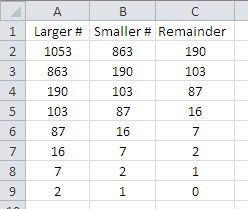
\includegraphics[width=2.5in]{images/gcd_spreadsheet.png}
\end{center}
\caption{Spreadsheet for computing gcd}\label{fig:gcd_spreadsheet}
\end{figure}


\subsection{Diophantine equations}\label{sec:diophantine}
%%% CPT start with the example.
Let's look now at another type of  problem, which has played a key role in the history of mathematics.

%Given two integers $a$ and $b$, the equation:
%\[ a m + b n = x\]
%where m and n are integers, the smallest value x can be is in fact the greatest common divisor of $a$ and $b$.  The way to find the values of $m$ and $n$ is to use the information from the process of finding the greatest common divisor.

\begin{example}{gcdintMultiples}
Find all integers $m$ and $n$ such that $16 m + 42 n = 8$.

To solve this, let us list each of the steps in finding the gcd of 42 and 16, as we explained in the previous section:
\[ 42 = (16)\cdot 2 + 10\]
\[ 16 = (10)\cdot 1 + 6\]
\[ 10 = (6)\cdot 1 + 4\]
\[ 6 = (4)\cdot 1 + 2\]
\[ 4 = (2)\cdot 2 + 0\]

Now let's start over again, but this time we'll keep track of what we're doing. If we start at the top of the list, but move the $16\cdot2$ to the other side of the equation, this yields:
\[ 42 \cdot 1 + 16 \cdot (-2) = 10.\]
Let's define a shorthand ``pair notation'' for the left-hand side. Let's represent any expression of the form $42\cdot x + 16 \cdot y$ as $(x,y)$. Using this rule, we denote $42 \cdot 1 + 16 \cdot (-2)$ by the pair $(1,-2)$.  Then our previous equation can represented  in ``pair notation'' as:
\[ (1,-2) = 10.\]
This ``vector notation'' can save a lot of writing over the course of a long computation.

Now consider the next equation down the list, which is 
$ 16 = (10)\cdot 1 + 6 $.
Using pair notation, we can write 16 with (0,1)  (since $16 = 42 \cdot 0 + 16 \cdot 1$). We've already seen that $10 = (1,-2)$, so we get:
\[(0,1) = (1,-2) + 6.\]
Now we can move the $(1,-2)$ to the left-hand side and subtract it from $(0,1)$ to get:
\[ (-1,3) = 6. \]
Now the next equation down the list is $10 = (6)\cdot 1 + 4$. 
Making similar replacements, we find:
\[(1,-2) = (-1,3) + 4\quad\Rightarrow\quad (2,-5) = 4.\]
Repeat again for the next equation down the list:
$ 6 = (4)\cdot 1 + 2$, which gives:
\[ (-1,3) = (2,-5) + 2 \quad\Rightarrow\quad (-3,8) = 2.\]  
At this point, we've gone as far as we can go.  (Verify this: what happens if you try to continue?) Now if we replace the pair notation $(-3,8)$ with what it originally represents, we get:
\[42\cdot ( -3) + 16 \cdot 8 = 2.\]
If we multiply this equation by 4, we have
\[42 \cdot( -12) + 16 \cdot 32 = 8.\]
It follows that $m=-12, n=32$ is an integer solution to our original equation, $16m + 42n = 8$.

Unfortunately we're not quite done yet, because we're supposed to find \emph{all} integer solutions. But we do have a particular solution, and we can leverage this information as follows.\footnote{What we're doing here  is a common ploy in mathematics.  We're using a \emph{particular} solution to reduce the problem to a \emph{homogeneous} equation (if you're not familiar with this terminology, then don't worry about it).  Exactly the same method is used in differential equations, and in linear algebra.}
   Suppose that $m,n$ is an arbitrary solution, so that  $42n + 16m = 8$.  We may subtract from this  equality the equation for the particular solution $m=-12, n=32$: 
\[\arraycolsep=1.4pt\def\arraystretch{1.3}
\begin{array}{rcrcl } 
    42n &~~+& 16m  &=& 8  \\
 -~ (42(-12) &~~+& 16(32)  &=&  8)   \\
    \cline{1-5} 
    42(n+12) &~~+& 16(m-32) &=& 0   
\end{array}
\]
Rearranging and dividing by common factors, we obtain:
\[ 21(n+12) = -8(m-32).\]
Now since the right-hand side is divisible by 8, then the left-hand side must also be divisible by 8.  This implies that $n+12$ must be divisible by 8, or 
\[ n+12 = 8k~~~(\text{for some integer}~k). \]
If we plug this in to the equation just above, we get:
\[ 21(8k) = -8(m-32),~~\text{or}~~m-32 = 21k .\]
We may rearrange to obtain finally:
\[ m = 32 + 21k ~~\text{and}~~ n = -12 + 8k~~~(\text{where }k \text{  is an arbitrary integer)} \]
as the most general solution to  $16m + 42n = 8$.
\end {example}

\begin{example}{}
We'll give another example, giving just the computations and no other words. We find integer solutions to $1053x + 863y =245$ as follows:
\begin{align*}
1053 = 863 + 190 &\implies 190 = (1,-1)\\
863 = 4 \cdot 190 +103 & \implies 103 = (0,1) - 4\cdot (1,-1) = (-4,5)\\
190 = 103 + 87 &\implies 87 = (1,-1) - (-4,5) = (5,-6)\\
103 = 87  + 16 &\implies 16 = (-4,5) - (5,-6) = (-9,11)\\
87 = 5 \cdot 16 + 7 &\implies 7 = (5,-6) - 5\cdot (-9,11) = (50,-61)\\
16 = 2 \cdot 7 + 2 &\implies 2 = (-9,11) - 2 \cdot(50,-61) = (-109,133)\\
7 = 3 \cdot 2 + 1 &\implies 1 = (50,-61) - 3 \cdot(-109,133) = (377 -460).
\end{align*}
This means that:  $377 \cdot 1053  - 460 \cdot 863 = 1$  (You may check this on a calculator.)  

\noindent
Now we may multiply both sides by 245, which gives:  
$$(245 \cdot 377)\cdot 1053 - (245 \cdot 460)\cdot 863 = 245.$$
Thus $x=(245 \cdot 377) =92365$ and $y=- (245 \cdot 460) =-112700$, so that
$$1053 \cdot 92365  - 863 \cdot 112700 = 245$$ 
is an integer solution.

To find \emph{all} integer solutions, we suppose that $(x,y)$ is an arbitrary solution to  $1053x + 863y = 245$. We can  subtract our computed solution to give:
$$1053(x-92365) + 863(y+112700) = 0,$$
or
$$1053(x-92365) = -863(y+112700).$$
Our computation shows that gcd(1053,863)=1, so by \emph{Euclid's Lemma} (Proposition~\ref{proposition:complex:EuclidLemma} in Chapter~\ref{complex}) and the left-hand side is divisible by 1053, so it must be the case that by $y + 112700$ is also divisible by 1053.  If we write $y + 112700 = 1053k$, it follows by algebra that $x - 92365 = -863k$. This means that 
$$ x = 92365 - 863k,~~ y = -112700 + 1053k$$
is the most general solution.  

This solution is correct, but we can simplify by shifting the value of $k$.  Note that $92365 = 107 \cdot 863 + 24$ and $112700 = 107 \cdot 1053 + 29$.  So we may replace $k$ with $(\ell + 107)$ to obtain:
$$ x = 92365 - 863(\ell + 107), y = -112700 + 1053(\ell + 107),$$
which after working out the algebra gives us:
$$ x = 24 + 863 \ell, y = 29 + 1053 \ell.$$
\end{example}
 
\begin {exercise}{}
Using the process above, find all integer solutions to the following equations.
\begin {enumerate} [(a)]
\item
$45m + 16n = 27$
\item
$360m + 14n = 32$
\item
$389m + 50n = 270$
\item
$4801m + 500n = 1337$
\item
$ 3524m + 7421n = 333$
\end {enumerate}
\end {exercise}

\begin{exercise}{DiophantineSS}
Modify the spreadsheet from Exercise~\ref{exercise:modular:Computer_exercise} to find the coefficients $n$ and $m$ such that $na + mb = \gcd(a,b)$ for given integers $a,b$.  Refer to Figure~\ref{fig:gcd_spreadsheet_with_coefs} for ideas.
\end{exercise}

\begin{figure}[h]
\begin{center}
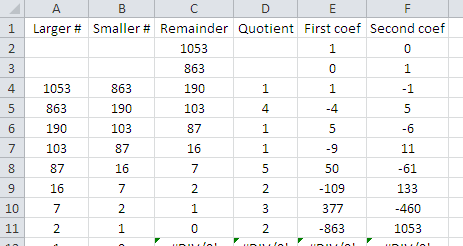
\includegraphics[width=4.5in]{images/gcd_spreadsheet_with_coefs.png}
\end{center}
\caption{Spreadsheet for computing gcd}\label{fig:gcd_spreadsheet_with_coefs}
\end{figure}


Do all  Diophantine equation have solutions? Let's investigate.

\begin {exercise}{diophant}
Explain why the following Diophantine equations have no integer solutions.
\begin {enumerate} [(a)]
\item
$2m + 4n = 1$
\hyperref[sec:modular_arithmetic:hints]{(*Hint*)}
\item
$3m + 27n = 2$
\end {enumerate}
\end {exercise}
The previous exercise shows that apparently not all Diophantine equations can be solved.  The following proposition shows which can and cannot be solved.

%We have shown that the gcd 
\begin{prop}{74}
A Diophantine equation of the form $an + bm = c$  has integer solutions for $n$ and $m$  if and only if $c$ is a multiple of the gcd of $a$ and $b$.
\end{prop}
\begin{proof}{}
Since this is an ``if and only if'' proof, we need to prove it both ways.  We'll do ``only if''  here, and leave the other way as an exercise.

Since we're doing the ``if'' part, we assume that $an + bm = c$ is solvable.
We'll represent the gcd of $a$ and $b$ by the letter $d$. Since gcd($a,b$) divides both $a$ and $b$, we may write $a = da'$ and $b = db'$ for some integers $a',b'$.  By basic algebra, we have $an+bm =d(a'n +b'm)$. If we substitute this back in the original Diophantine equation, we get:
\[d(a'n +b'm)=c\]
It follows that $c$ is a multiple of, $d$, which is the gcd of $a$ and $b$.
\end{proof}

\begin {exercise}{prop74}
Prove the ``if'' part of Proposition~\ref{proposition:modular:74}. 
\hyperref[sec:modular_arithmetic:hints]{(*Hint*)}
\end{exercise}


%Now we have the info to prove which modular equations have a solution.
At the beginning of this section, we ``introduced'' Diophantine equations.  But we have seen them before:

\begin{exercise}{}
\begin{enumerate}[(a)]
\item
Find the general solution to: $242m + 119n = 53$.
\item 
Use your solution to solve the modular equation: $242x \equiv 53 \pmod{119}$.
\item
Use your solution to solve the modular equation:  $119y \equiv 53 \pmod{242}$.
\end{enumerate}
\end{exercise}
This example shows that Diophantine equations are just modular equations in a disguised form!  Furthermore, each Diophantine equation is associated with \emph{two} modular equations:

\begin{exercise}{}
Given that $(m,n)$ is a solution to $a \cdot m + b \cdot n  = c$, give (a) a modular equation involving $a,b,c$ that $m$ satisfies; and (b) a modular equation involving $a,b,c$ that $n$ satisfies.
\end{exercise}


In Example~\ref{example:modular:speed_up2}, we saw that not all equations of the form $ax \equiv c \pmod b$ have an answer.  We  now have the means to determine which modular arithmetic equations have an answer:

\begin{prop}{mod_eq_solution} 
Given the equation $ax \equiv c\pmod{b}$, where $a,b,c$ are all given integers and $x$ is the variable we're solving for, one can find an integer answer for $x$ if and only if $c$ is an integer multiple of the greatest common divisor of $a$ and $b$.  
\end{prop}

\begin {exercise}{propiff}
Prove both the ``if''  and the ``only if'' parts of Proposition~\ref{proposition:modular:mod_eq_solution}.
\hyperref[sec:modular_arithmetic:hints]{(*Hint*)}
\end{exercise}


\begin{exercise}{}
Which of the following equations have integer solutions? If solutions exist, find them all. If no solutions exist, prove it!
\begin{enumerate}[(a)]
\item
$15x = 3 \pmod{12}$
\item
$4x = 17 \pmod{23}$
\item
$503x = 919 \pmod{1002}$
\item
$504x = 919 \pmod{1002}$
\end{enumerate}

\end{exercise}

To close off this section, we take care of some unfinished business. Way back when we were showing the existence of irrational numbers, we made use of \emph{Euclid's Lemma} (Proposition~\ref{proposition:complex:EuclidLemma} in Chapter~\ref{complex}). We weren't able to give a real proof then--but we're able to now, thanks to Proposition~\ref{proposition:modular:74}:\index{Euclid's lemma!proof}

\begin{exercise}{EuclidLemmaProof}
\begin{enumerate}[(a)]
\item
Let  $p$ be a prime, and let  $a$ be an integer.  Show that $a$ is relatively prime to $p$  if and only if there exist integers $m$ and $n$ such that $pm + an=1$.
\hyperref[sec:modular_arithmetic:hints]{(*Hint*)}
\item
Suppose $p$ is prime, and suppose $a$ is relatively prime to $p$.  Suppose also that $p$ divides $ab$. By multiplying the equation in part (a) by $b$, show that $p$ must divide $b$.
\hyperref[sec:modular_arithmetic:hints]{(*Hint*)}
\item
Prove \term{Euclid's Lemma}:  Let $p$ be a prime number, and let $a$ and $b$ be integers. If $p$ divides $ab$, then either $p$ divides $a$ or $p$ divides $b$.
\hyperref[sec:modular_arithmetic:hints]{(*Hint*)}
\end{enumerate}
\end{exercise}


\subsection{Multiplicative inverse for modular arithmetic\label{subsec:MultInve}}
This section is supposed to be about modular division, but so far we've been talking about all kinds of other stuff. You may be wondering, So where's the modular division? You're about to find out!

Recall that the set $Z_n$ under the operation $\oplus$ forms a group:  
it has closure, it's associative, it has an additive identity, and all elements have inverses.  On the other hand $Z_n$ does not form a group under $\odot$ for any $n \ge 2$.  


Why is this? Because the inverse property fails for the element 0. The multiplicative identity must be 1, yet $0\cdot m \neq 1$ for all $m\in Z_n$.

But let's not give up so easily in our quest to form multiplicative groups. Since it appears that 0 is a problem, suppose we take all the elements of $Z_n$ \emph{except} 0? We write the set of nonzero elements of $Z_n$ as $Z_n \setminus \{0\} $. Let's see whether this a group under $\odot$. We remind you that $a \odot b$  is defined by: $a \odot b = r$ where $a,b,r\in Z_n$ and $a \cdot b = kn + r$ where $k$ an integer.)


%look at modular chapter to avoid repetition.  Use a Cayley table for multiplication proof.
\begin{example}{Groupornot3}
The Cayley table for $Z_3 \setminus \{0\}$ is:


\begin{tabular}{ l | r r  }
  $\odot$ & 1 & 2 \\
  \hline
  1 & 1 & 2 \\
  2 & 2 & 1 \\
\end{tabular}


Notice that each column has 1, meaning that each element has an inverse.  It is also closed, associative and has an identity. Thus $Z_3 \setminus \{0\}$ is a group under $\odot$.  
\end{example}

% However not all sets of $Z_n$ are a group under multiplication.

\begin{example}{Groupornot4}
The Cayley table for $Z_4 \setminus \{0\}$ is


\begin{tabular}{ l | r r r }
  $\odot$ & 1 & 2 & 3\\
  \hline
  1 & 1 & 2 & 3\\
  2 & 2 & 0 & 2\\
  3 & 3 & 2 & 1\\
\end{tabular}

Notice that the 2 column does not have a 1 in it, meaning that 2 does not have an inverse in $Z_4$. Thus, $Z_4 \setminus \{0\}$ is not a group under $\odot$.
\end{example}

The fact that 2 has no inverse is due to 2 being a divisor of 4.  This makes all integer multiples of 2 to cycle between the values 0 and 2 $\pmod 4$. 

%If any of the numbers in the set $Z_n$ can evenly divide $n$, then the same problem will occur.  It follows that any $n$ that is not divisible by any integer from 1 to $n$ should form a group $Z_n\setminus \{0\}$.

\begin{example}{Finding a larger multiplicative inverse}

%Start with 3k = 1 mod 31 => 3k - 1 = 31n => 3k - 31n = 1;

Finding the multiplicative inverse in $Z_n \setminus \{0\}$ for small values of $n$  is not difficult.  But what about finding the multiplicative inverse of 3 in $Z_{31}\setminus \{0\}$?  

%%% CPT I think the following discussion has some problems.
% 
% Start by finding an integer $k$ such that $31 < 3 \cdot k < 31 + 3$.  In this case:
 % \[31 < 3 \cdot 11  = 33 < 31+3 = 34\] 

 % Then subtract 31 from $3 \cdot 11$ to yield 2. Now find an integer $j$ such that
% $31 < 2+ 3\cdot j < 31 + 33$ in this case $j=10$ yielding:
% \[31 < 2+ 13\cdot 10 = 32 < 31 + 3\]

% Then subtract 31 from $2+3 \cdot 10$ to yield 1. Now we add the integers $j$ and $k$ together.  
% \[j+k = 21\]
% Applying the definition of modular multiplication we get:
% \[3 \cdot 21 - 31 \cdot 2 = 63 - 62 = 1\]

% This is just a repeat of the 2 sticks method.  and suffers from the problem that it may need to be repeated $n$ times to find the multiplicative inverse, and it needs to be repeated $n$ times to show that no inverse exists.
% \end{example}

% \begin{example}{A better way of finding larger multiplicative inverses}
% Using modular arithmetic, we can find a solution more efficiently.  Take the same example of finding the multiplicative inverse of 3 in $Z_{31}$.  

Really all we're looking for is a number $k$ such that $3k \equiv 1 \pmod {31}$.  Since 31 is prime, it must be relatively prime to 3, meaning the gcd of 31 and 3 must be 1.  1 is a multiple of 1, so there is a solution and in fact this is just a special case of an earlier proposition.  We convert it to a Diophantine equation:
\[3k + 31j = 1\]
Using the gcd algorithm, we find:
\[31+3\cdot(-10) = 1,\]
and applying $\pmod{31}$ gives
\[3\cdot(-10) \equiv 1 \pmod{31}.\]
Finally, we use the definition of modular arithmetic to convert $-10$ into a member in $Z_{31}$:
\[3\cdot(21) \equiv 1 \pmod{31}.\] 
\end{example}


\begin{exercise}{90}
Prove or disprove that the following sets form a group by either finding a multiplicative inverse for all members, or by finding a member that does not have a multiplicative inverse.
\begin{enumerate}[(a)]
\item
$Z_5\setminus \{0\}$
\item
$Z_7\setminus \{0\}$
\item
$Z_9\setminus \{0\}$
\item
Make a conjecture for which sets $Z_n \setminus \{0\}$ form a group under multiplication.
\end{enumerate}
\end{exercise}

%let a < p, a has an inverse when there is a solution to the diophantine equation ak - pn = 1; When a and p are relatively prime, then there is a solution to the diophantine equation.  Solve for integer, set modp, replace k with remainder mod p.
%Using earlier proposition for ax=cmodb and state this is just a special case.

\begin{prop}{Groupornotp}
All elements in $Z_p \setminus \{0\}$ have an inverse under multiplication mod $p$. 
\end{prop}
\begin{proof}
Let $a,p$ be known integers where $a < p$ and $p$ is prime.  There exists an inverse to $a$ under multiplication $\pmod p$ when there is a solution $k$  to the equation $ak = 1 \pmod p$ where $k$ is an integer.  By Proposition~\ref{proposition:modular:mod_eq_solution}, this equation can be solved if and only if the gcd of $a$ and $p$ is equal to 1.  Since $p$ is prime and $a<p$ then the gcd of $a$ and $p$ must be 1.
\end{proof}

\begin{prop}{Units}
An element $a$ of  $Z_p \setminus \{0\}$ have an inverse under multiplication mod $p$ if and only if gcd($a,p$)=1  (that is, $a$ is relatively prime to $p$).
\end{prop}
The proof of this proposition is up to you:

\begin{exercise}{93}
Prove both the ``if'' and ``only if'' parts of Proposition~\ref{proposition:modular:Units}.
\hyperref[sec:modular_arithmetic:hints]{(*Hint*)}
\end{exercise}

\begin{exercise}{94}
Show that if $n$ is not prime, then $Z_n\setminus \{0\}$ is not a group under multiplication.
\hyperref[sec:modular_arithmetic:hints]{(*Hint*)}
\end{exercise}

\subsection{Chinese remainder theorem}
We now are experts at finding solutions to congruences  of the form $ax \equiv c \pmod b$. But what about multiple congruences?  Take for example:

\[x \equiv 4 \pmod 7; \qquad x \equiv 5 \pmod 9.\]

Can we find  an $x$ that solves both at the same time? 

The first-century Chinese mathematician Sun Zi considered problems like this, and was able to come up with a general method of solution. His result is now known as the \term{Chinese Remainder Theorem}.\index{Chinese Remainder Theorem}  

We may apply Sun Zi's solution (expressed in modern algebraic language) to our particular case as follows. For the first congruence we have the general solution $x=4+7k$, where $k$ is any integer in $\mathbb{Z}$.  If we  substitute $4+7k$ for $x$ in the second congruence, we get:
\[4+7k \equiv 5 \pmod 9 \implies 7k \equiv 1 \pmod 9.\]
At this point we could use the Euclidean algorithm to find $k$. But it's often easier to use the trial-and-error methods that we developed earlier. In this case, the method amounts to adding multiples of 9 to the right-hand side until you get something that is divisible by 7.  In this case, we find:
\[7k \equiv 1 + 3\cdot 9 \pmod 9 \implies 7k \equiv 28 \pmod 9 \implies k \equiv 4 \pmod 9.\]
This means $k = 9j + 4$ for some integer $j$.  We substitute $9j + 4$ for $k$ back into $x=4+7k$ to get:
\[x = 4 + 7(9j + 4) = 4 + 63j + 28 = 32 + 63j.\]
So the answer must be $x \equiv 32 \pmod {63}$  When we check, $32 = 9 \cdot 3 + 5 = 7 \cdot 4 + 4$ and $95 = 9 \cdot 10 + 5 = 7 \cdot 13 + 4$ and indeed that is the case.  Notice the ending modulus was the least common multiple of the first and second modulus (7 and  9, respectively) in the original set of modular equations.


Now, not all multiple congruences have an answer.  Take the following pair of congruences:
\[x \equiv 3 \pmod 4; \qquad x \equiv 4 \pmod 6.\]
We follow the same pattern.  There is a solution for the first congruence $x = 4k + 3$ where $k$ is any integer.  Plug this into the second congruence to yield:
\[4k + 3 \equiv 4 \pmod 6 \implies 4k \equiv 1 \pmod 6.\]
From the Euclidean algorithm, we know there is a solution to this congruence if and only if gcd$(4,6) = 1$, but we know gcd$(4,6) = 2$.  Therefore there is no solution.  


\begin{exercise}{}
Solve the following pairs of congruences or show that they do not have a solution:
\begin {enumerate}[(a)]
\item
$x \equiv 2 \pmod{3}; \quad x \equiv 3 \pmod{4}.$
\item
$x \equiv 12 \pmod{23}; \quad x \equiv 7 \pmod{11}.$
\item
$x \equiv 3 \pmod{13}; \quad x \equiv 20 \pmod{31}.$
\item
$x \equiv 2 \pmod{6}; \quad  x \equiv 56 \pmod{72}.$
\end {enumerate}
\end {exercise}

\begin {exercise}{congruence}
\begin{enumerate}[(a)]
\item
Find a pair of congruences of the form: $x \equiv a \pmod{9};~~x \equiv b \pmod{15}$ that no common solution.
\item
Show that \emph{any} pair of congruences of the form 
\[ ax \equiv b \pmod{3}; \qquad cx \equiv d \pmod{7} \]
 will have a common solution.
\item
*Prove the following: Given a pair of congruences
\[ ax \equiv b \pmod{m}; \qquad cx \equiv d \pmod{n} \]
 which both have solutions, such that gcd($m,n$)=1. Then the congruences also have a common solution.
 \hyperref[sec:modular_arithmetic:hints]{(*Hint*)}
\item
*Prove the following: Given a pair of congruences
\[ x \equiv b \pmod{m}; \qquad x \equiv d \pmod{n}. \]
 such that gcd($m,n$)=1. Then there exist common solutions to both congruences; and all common solutions are congruent mod $mn$.
\end{enumerate}
\end{exercise}


We can use the same method to solve any number of simultaneous congruences. Take for example:

\[x \equiv 4 \pmod 7; \quad x \equiv 5 \pmod 9; \quad x \equiv 1 \pmod 2.\]

From the above example we know the general solution for the first two congruences  is $x \equiv 32 \pmod {63}$.  So we need to solve:
\[x \equiv 32 \pmod {63}; \qquad x \equiv 1 \pmod 2\]
We solve this by the same process as before: 
\begin{align*}
x = 1 + 2k &\implies 1 + 2k \equiv 32 \pmod {63} \implies 2k \equiv 31 \pmod {63}\\
&\implies 2k \equiv 31+63 \pmod {63} \implies 2k \equiv 94 \pmod {63} \\
&\implies k \equiv 47 \pmod {63}.
\end{align*}

Substitute to obtain $x = 1 + 2(47+ 63j) = 95 + 126j \equiv 95 \pmod{126}.$.  


\begin{exercise}{}
Solve the following sets of congruences or show that they do not have a solution:
\begin {enumerate}[(a)]
\item
$x \equiv 2 \pmod{3}; \quad x \equiv 3 \pmod{4}; \quad x \equiv 4 \pmod{5}.$
\item
$x \equiv 12 \pmod{23}; \quad x \equiv 7 \pmod{11}; \quad x \equiv 3 \pmod{4}.$
\end {enumerate}
\end {exercise}






